\documentclass[12pt]{report}
\usepackage{graphicx}
\usepackage[czech]{babel}
\usepackage[utf8]{inputenc}
\usepackage{titling}
\usepackage{pdfpages}
\usepackage[nopar]{lipsum}
\usepackage{mathtools}
\usepackage{multirow}
\usepackage{caption}
\usepackage{float}
\usepackage{enumitem}
\usepackage{listings}
\usepackage{amsmath}
\usepackage{amssymb}
\setlength{\parindent}{1cm}
\setlength{\hoffset}{-1.1cm} 
\setlength{\voffset}{-2cm}
\setlength{\textheight}{23.0cm} 
\setlength{\textwidth}{15cm}

\begin{document}
\title{Bakalářská práce}
\author{Lukáš Kuhajda}
\date{Akademický rok 2018/2019}
\begin{titlepage}
	\begin{center}
		
\includegraphics[scale=0.5]{logo_zcu}\\
		\vspace{5cm}
		\begin{Large}
			\textbf{\thetitle}\\
		\end{Large}
		
		\vspace{3cm}
		\theauthor\\
		\vspace{5cm}
		\thedate
	\end{center}
\end{titlepage}
\newpage	
	
\tableofcontents
\newpage





\chapter{Úvod}
Tato práce je věnována systémům, které pomocí měření z LIDARu (Light Detection And Ranging) utváří mapu prostředí, v němž se pohybují. První část práce je zaměřena obecně na problém simultánní lokalizace a mapování (SLAM). Mobilní robot je umístěn do neznámého prostředí a jeho úkolem je určovat svoji pozici a utvářet mapu. Jsou zde popsány vnitřní principy a různé přístupy k řešení problému. Daná tématika momentálně vstupuje do podvědomí i širší veřejnosti, neboť pomalu dochází k přechodu na autonomní vozidla, která fungují na podobných principech. Tyto automobily však využívají i mnoho dalších senzorů, jako jsou například kamery. V této práci je zaměření čistě na systémy využívající 2D LIDAR, tedy sezor, měřící vzdálenosti pouze v jedné výškové úrovni.\\
\indent Další kapitola se věnuje třem nejrozšířenějším 2D SLAM systémům, přesněji se jedná o gMapping, HectorSLAM a Google Cartographer. Je zde popsáno, na jakých principech každý ze systémů pracuje a jak je daný přístup do systému implementován. \\
\indent Třetí kapitola je zaměřena již na porovnání daných systémů na základě naměřených dat. Nejprve je zde popsán operační systém pro roboty (ROS), ve kterém pracují všechny tři systémy a pomocí kterého se nahrávala reálná data. V další části je ukázáno, jak byla získána data. V této práci jsou použity tři typy dat, kdy jsou využity čistě simulační data, která jsou nahraná pomocí již zmíněného operačního systému pro roboty. Dále data nahraná na univerzitě MIT v Massachusetts a jako poslední data nahraná mobilním robotem přímo v budově FAV na Západočeské univerzitě v Plzni. Dále je zde rozebráno, jak data byla zpracována, aby byla připravena na následné porovnávání. Poslední částí této kapitoly je srovnání výsledků. Je zde uvedeno, jaké kritérium bylo pro srovnávání zvoleno. Dále jsou zde popsány získané výsledky pro jednotlivé datasety. U každého typu dat je také vyhodnocení, jaká metoda se pro daná data hodila nejvíce, jak si vedly metody ostatní a důvody, proč tomu tak bylo.\\
\indent V páté kapitole je uvedení bližšího průzkumu vybraného systému. Jsou zde popsány důvody, které vedly k vybrání zvoleného systému. Pro náhled do vnitřních pochodů, jsou zde také uvedena srovnání, jak metoda proběhne při změně určitých nastavitelných parametrů. Následně je pro každou změnu zhodnoceno, jaký vliv na systém daná změna má a proč tomu tak je. Nakonec je uvedeno, jaké změny by bylo vhodné v systému udělat. Jedná se jak o změny zlepšující výkonnost systému, tak i o změny pouze ulehčující práci pro uživatele.\\
\indent Poslední kapitolou je závěr, ve kterém je zhodnocena postupně celá práce. Hlavním zaměřením je zde popis práce s jednotlivými metodami, jak složité je bylo nastavovat, jaká k nim byla dokumentace a jak její nedostatky doplňovala komunita a především, jak byly systémy po celou dobu práce s nimi stabilní, či nestabilní.

\newpage

\chapter{Simultánní lokalizace a mapování}

V této sekci se nachází seznámení s problémem simultánní lokalizace a mapování. Je zde probírána jak historie, tak struktura algoritmů, na kterých jsou založeny jednotlivé systémy řešící problém SLAM. 

\section{Historie}
Za počátek diskuze problému se považuje konference Robotics and Automation Conference, konaná v roce 1986. Pravděpodobnostní metody byly tehdy ještě velmi nerozvinuté, jak v robotice, tak i v umělé inteligenci. Došlo tedy pouze k debatě na dané téma.\\
\indent K většímu posunu kupředu se dostalo o pár let později, kdy vyšla práce pojednávající o vztahu mezi orientačními body (landmarky) a snížením geometrické nepřesnosti. Důležitým poznáním bylo zjištění, že mezi odhady landmarků na mapě je velká korelace, která je rostoucí s dalšími pozorováními.[1]\\
\indent Ve stejném období vznikaly základy vizuální navigace a navigace pracující se sonarem s použitím Kalmanova filtru. Práce byly v základu podobné. Ukazovaly, že odhady landmarků získané pohybem robota prostředím, jsou v korelaci s ostatními kvůli chybě v odhadu pozice robota [2]. Je tak třeba mít stav složený z pozice robota a landmarků, tím však vznikal velký stavový vektor s náročností rostoucí v kvadrátu. V daném období byla tendence snižovat korelaci landmarků.\\
\indent Později došlo k sjednocení problémů lokalizace a mapování a závěru, že snaha minimalizovat korelaci mezi landmarky byla chybná. Naopak bylo v zájmu korelaci co nejvíce zvýšit. Struktura SLAMu, a celkově první použití tohoto akronymu, byla prezentována v roce 1995 na International Symposium of Robotics Research (ISRR)[3]. Poté se v roce 1999 na ISRR odehrálo první zasedání pojednávající přímo o SLAM a došlo k představení práce dosahující dostatečné konvergence mezi SLAMem využívající Kalmanův filtr a pravděpodobnostními metodami pro lokalizaci a mapování.[4]


\section{Formulace a struktura} 
Jedná se o proces, při kterém robot vytváří mapu prostředí v němž se pohybuje a na základě mapy určuje svoji pozici v prostoru. Pro určování trajektorie robota a rozložení landmarků není třeba předchozí znalosti jeho lokace, neboť odhad těchto parametrů probíhá v reálném čase. 

\begin{figure}[!ht]
	\begin{center}
		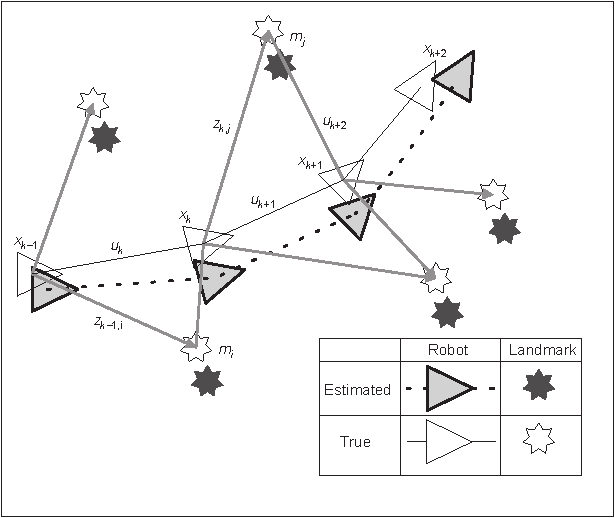
\includegraphics[width=0.6\columnwidth]{imgs/SLAM_estimate_vs_reality.pdf}
	\end{center}
	\caption{Znázornění chyby v odhadu pozice a landmarků (z [5]).}
	\label{fig:SLAM_estimate_vs_reality}
\end{figure}

\subsection{Pravděpodobnostní SLAM}
Cílem je získat v časovém okamžiku k odhadu hustoty pravděpodobnosti
\begin{equation}
	P(\textbf{x}_k,\textbf{m}|\textbf{Z}_{0:k},\textbf{U}_{0:k},\textbf{x}_0)
\end{equation}
pro každý časový okamžik ${k}$, kde $\textbf{x}_k$ je stavový vektor popisující pozici a orientaci robota, $\textbf{m}$ je množina landmarů, tedy mapa, $\textbf{Z}_{0:k}$ jsou všechna pozorování landmarků, $\textbf{U}_{0:k}$ je historie vstupů a $\textbf{x}_0$ je počáteční stav. Jedná se tedy o srduženou posteriorní hustotu mapy, stavu vozidla s ohledem na zaznamenané pozorování, řídící vstupy a  počáteční stav robota. Pro výpočet je využit Bayesův teorém, který vyžaduje rozdělení algoritmu do dvou kroků. Prvním krokem je predikce, která využívá model pohybu robota. Tím druhým je korekce modelu pozorování, ke kterému jsou třeba data ze senzorů. Pohybový model a model pozorování tak popisují vliv vstupního řízení a pozorování.\\
\indent Model pozorování popisuje pravděpodobnost zisku pozorování $\textbf{z}_k$, pokud je známa poloha vozidla $\textbf{x}_k$ a landmarků $\textbf{m}$.
\begin{equation}
	P(\textbf{z}_k|\textbf{x}_k,\textbf{m})
\end{equation} 
\indent Model pohybu vozidla může být popsán jako stavový přechodový model. \\Přechodový stav je předpokládán jako Markovův proces, při kterém následující stav $\textbf{x}_k$ je závislý pouze na předchozím stavu $\textbf{x}_{k-1}$ a aplikovaném řízení $\textbf{u}_k$ a není tak závislý ani na mapě, ani na pozorování.
\begin{equation}
	P(\textbf{x}_k|\textbf{x}_{k-1},\textbf{u}_k)
\end{equation}
Implementace je tak ve formě dvoukrokého rekurzivního algoritmu.\\
\\
Aktualizace času (predikce):
\begin{equation}
	\begin{split}
	P(\textbf{x}_k,\textbf{m}|\textbf{Z}&_{0:k-1},\textbf{U}_{0:k},\textbf{x}_0)=\\&\int P(\textbf{x}_k|\textbf{x}_{k-1},\textbf{u}_k)\times P(\textbf{x}_{k-1},\textbf{m}|\textbf{Z}_{0:k-1},\textbf{U}_{0:k-1},\textbf{x}_0)d\textbf{x}_{k-1}
	\end{split}
\end{equation}
\\
Aktualizace měření (korekce):
\begin{equation}
	P(\textbf{x}_k,\textbf{m}|\textbf{Z}_{0:k},\textbf{U}_{0:k},\textbf{x}_0)=\frac{P(\textbf{z}_k|\textbf{x}_k,\textbf{m})P(\textbf{x}_k,\textbf{m}|\textbf{Z}_{0:k-1},\textbf{U}_{0:k},\textbf{x}_0)}{P(\textbf{z}_k|\textbf{Z}_{0:k-1},\textbf{U}_{0:k})}
\end{equation}

\subsection{Struktura}
Model pozorování udává závislost polohy vozidla a pozice landmarků, z čehož vyplývá, že sdružená posteriorní pravděpodobnost nemůže být rozdělena na
\begin{equation}
	P(\textbf{x}_k,\textbf{m}|\textbf{z}_k)\neq P(\textbf{x}_k|\textbf{z}_k)P(\textbf{m}|\textbf{z}_k),
\end{equation}
neboť by to vedlo k chybným odhadům. Dalším zdrojem chyb je špatný odhad pozice robota. Landmarky jsou ale silně korelované, takže chybný odhad landmarku vůči mapě nevede k chybné poloze dvou landmarků navzájem.\\
\indent Velmi důležitým poznatkem bylo zjištění, že korelace mezi landmarky monotónně vzrůstá s počtem jejich pozorování (dokázáno pouze pro lineární Gaussovský případ [6]). Odhad pozice landmarku je tedy s narůstajícím počtem pozorování monotónně přesnější. Tento jev nastává díky, v podstatě, skoro nezávislému měření relativních pozic mezi landmarky. Ty jsou zcela nezávislé na natočení vozidla a úspěšné pozorovnání z tohoto bodu může nést další nezávislá měření relativních rozložení landmarků. \\
\indent Pohybem v prostoru, robot získává pozorováním novou pozici známých landmarků vůči sobě a dle této informace aktualizuje jejich pozici a též svoji odhadovanou polohu. Pokud již nějaký landmark není pozorován, tak je jeho pozice aktualizována dle změny pozorovaných landmarků. Při pozorování nových landmarků dochází ke korelaci s již známými, čímž se vytváří síť. Čím častěji jsou dva landmarky pozorovány při jednom měření, tím je síla korelace větší. Opětovným projížděním prostředím je tak získána přesnější a robustnější mapa. Například násobným průchodem jedné smyčky se získá znatelně kvalitnější záznam o daném prostředí, než pouze jedním projetím.\\

\begin{figure}[!ht]
	\begin{center}
		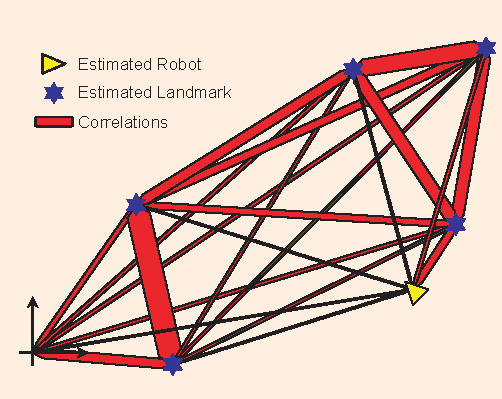
\includegraphics[width=0.6\columnwidth]{imgs/SLAM_corelations.pdf}
	\end{center}
	\caption{Znázornění korelací mezi landmarky a robotem (z [5]).}
	\label{fig:SLAM_corelations}
\end{figure}

\newpage
\section{Řešení problému SLAM}
Při řešení je potřeba adekvátně obsáhnout jak složku modelace prostředí, tak i tvorbu pohybového modelu.
Je řada možností jak tento problém řešit, například princip Monte Carlo, kdy se rozdělují hustoty pravděpodobnosti odhadu pozice robota. Další možností je Markovova lokalizace, jedná se o pravděpodobnostní formu SLAM. Nejčastější reprezentace problému ve formě stavového modelu zatíženého šumem, což vede k použití rozšířeného Kalmanova filtru (v originále $extended$ $Kalman$ $filter\rightarrow EKF$). Možností je ještě rozčlenění pohybového modelu vozidla na vzorky s obecnějším negausovským rozdělením pravděpodobnosti. V tomto případě je řeč o použití Rao-Blackwellizovaného částicového filtru. Dalším rozšířeným způsobem je Graph-based SLAM, kde jsou pozice robota vůči sobě poskládány v grafu a následně zpětně optimalizovány. 
\\
\subsection{EKF-SLAM}
EKF-SLAM je třída algoritmů využívající $extended$ $Kalman$ $filter$. Rozšířený Kalmanův filtr je implementací Bayesovské statistiky, která pracuje s gaussovským nelineárním systémem. \\
Pohyb robota je zde popsán rovnicí
\begin{equation}
	P(\textbf{x}_k|\textbf{x}_{k-1},\textbf{u}_k)\leftrightarrow \textbf{x}_k=\textbf{f}(\textbf{x}_{k-1},\textbf{u}_k)+\textbf{w}_k,
\end{equation} 
kde $\textbf{f}(\textbf{x}_{k-1},\textbf{u}_k)$ je funkce modelující pohyb robota a $\textbf{w}_k$ jsou chyby měření.\\
\\
Model pozorování je vyjádřen vztahem
\begin{equation}
	P(\textbf{z}_k|\textbf{x}_k,\textbf{m})\leftrightarrow \textbf{z}_k=\textbf{h}(\textbf{x}_k,\textbf{m})+\textbf{v}_k
\end{equation}
kde funkce $\textbf{h}(.)$ popisuje geometrické vlastnosti pozorování a $\textbf{v}_k$ jsou chyby měření.
Tyto dvě definice jsou využity v metodě EKF k výpočtu průměru a kovariance sdruženého posteriorního rozložení\\
\indent průměr:
\begin{equation}
	\begin{bmatrix}
	\hat{\textbf{x}}_{k|k}\\\hat{\textbf{m}}_k
	\end{bmatrix}=E
	\begin{bmatrix}
	\textbf{x}_k |\textbf{Z}_{0:k}\\\textbf{m}\indent
	\end{bmatrix}
\end{equation}

\indent kovariance:
\begin{equation}
	\textbf{P}_{k|k}=\begin{bmatrix}
	\textbf{P}_{xx} \textbf{P}_{xm}\\\textbf{P}^T_{xm} \textbf{P}_{mm}
	\end{bmatrix}_{k|k}=E\begin{bmatrix}
	\begin{pmatrix}
	\textbf{x}_k-\hat{\textbf{x}}_k\\\textbf{m}-\hat{\textbf{m}}_k
	\end{pmatrix} \begin{pmatrix}
	\textbf{x}_k-\hat{\textbf{x}}_k\\\textbf{m}-\hat{\textbf{m}}_k
	\end{pmatrix}^T |\textbf{T}_{0:k}
	\end{bmatrix}
\end{equation}
Aktualizace času je pak počítána jako
\begin{equation}
\textbf{\^{x}}_{k|k-1}=\textbf{f}(\textbf{\^{x}}_{k-1|k-1},\textbf{u}_{k})
\end{equation}
\begin{equation}
	\textbf{P}_{xx,k|k-1}=\triangledown\textbf{f}\textbf{P}_{xx,k-1|k-1}\triangledown\textbf{f}^T+\textbf{Q}_k,
\end{equation}
kde $\triangledown\textbf{f}$ je Jacobián z funkce $\textbf{f}$, která vychází z odhadu stavu $\textbf{\^{x}}_{k-1|k-1}$.\\
\indent Aktualizace pozorování se provádí výpočtem rovnic
\begin{equation}
	\begin{bmatrix}
	\hat{\textbf{x}}_{k|k}\\\hat{\textbf{m}}_k
	\end{bmatrix}=
	[\textbf{\^{x}}_{k|k-1}\textbf{\^{m}}_{k-1}]+\textbf{W}_{k}[\textbf{z}_k-\textbf{h}(\textbf{\^{x}}_{k|k-1},\textbf{\^{m}}_{k-1})]
\end{equation}
\begin{equation}
	\textbf{P}_{k|k}=\textbf{P}_{k|k-1}-\textbf{W}_k\textbf{S}_k\textbf{W}^T_k,
\end{equation}
kde 
\begin{equation}
	\textbf{S}_k=\triangledown\textbf{h}\textbf{P}_{k|k-1}\triangledown\textbf{h}^T+\textbf{R}_k
\end{equation}
\begin{equation}
	\textbf{W}_k=\textbf{P}_{k|k-1}\triangledown\textbf{h}^T\textbf{S}^{-1}_k,
\end{equation}
přičemž $\triangledown\textbf{h}$ je Jacobián z funkce $\textbf{h}$, která vychází z odhadu stavu $\textbf{\^{x}}_{k|k-1}$ a odhadu mapy $\textbf{\^{m}}_{k-1}$.\\
\indent Mezi hlavní problémy této metody se řadí konvergence, výpočetní složitost, asociace dat a nelinerita. Kvůli nelinearitě může dojít k větším nepřesnostem ve výsledku, neboť EKF-SLAM využívá lineárních modelů pro vyjádření nelineárního pohybu a modelu pozorování. Konvergence a konzistence modelu je tedy jistá pouze v lineárním případě. 

\subsubsection{Výpočetní složitost}
Jedním ze základních kritérií všech algoritmů je jejich výpočetní složitost. Je tak třeba co nejvíce zjednodušit sdružený stav z pozice robota a landmarků a operace s nimi. Základním rozdělením metod redukujících výpočetní složitost, je rozlišování optimálních, konzervativních a nekonzistentních metod.\\ 
\indent První typ, optimální metody, jsou založené na redukci daného výpočtu. Rovnicí pro aktualizaci pozorování omezují požadované výpočty. Výsledkem jsou pak odhady a kovariance, stejně tak, jako je tomu v případě plnohodnotné formy SLAM. U metod konzervativních dochází k reformulaci stavového prostoru do informační podoby. To umožňuje rozdělení výsledné matice s informacemi, což vede ke snížení výpočtů, ale také k odhadům s vyšší neurčitostí nebo kovariancí. Konzervativní metody jsou nejčastěji implementovány v reálném použití, neboť dostatečně redukují výpočetní nároky a stále udržují dostatečnou odhadovací schopnost. Poslední možností jsou nekonzistentní metody. Jedná se o algorithmy, které mají nižší neurčitost nebo kovarianci, než algoritmy optimální. Pro řešení SLAM v praxi se ale nepoužívají.

\subsubsection{Oddělné aktualizace}
Metody využívající oddělěné aktualizce vytvářejí optimální odhady. Při implementaci základní podoby aktualizace pozorování, se při každém novém měření aktualizuje jak stav vozidla, tak i mapy. To vede ke kvadratickému nárůstu složitosti s množstvím landmarků. Při této implementaci se však mapa rozdělí na submapy.\\
\indent Rozlišují se dva způsoby možné implementace. První z nich pracuje na zmenšené oblasti, ale stále si drží globální referenční souřadnice, jedná se například o algoritmus $compressed$ $EKF$ (CEFK). Druhou možností je tvorba menších map s vlastním\\ souřadnicovým rámcem neopouštějícím danou submapu. Jsou to algorithmy $constrained$ $local$ $submap$ $filter$ (CLSF, v překladu - omezený lokální submapový filtr). Pro další rozbor je vhodnější druhá možnost, neboť je jednodušší a při provádění operací s velkou frekvencí opakování je méně ovlivněna linearizačními chybami. Je také stabilnější a zabraňuje příliš velkému nárůstu globální kovariance. \\
\indent Logaritmus submapy se skládá z dvou nezávislých odhadů, které si stále udržuje. Jde o vektory $x_G$ a $x_R$, kdy $x_G$ je mapa složená z globálně referencovaných landmarků a globálně referencované pozice dané submapy a $x_R$ je lokální submapa s lokálně referencovanou pozicí robota a lokálně referencovanými landmarky. Při získání pozorování se aktualizují pouze landmarky náležící aktuální submapě, ve které se robot nachází. Celkový globální odhad je pak získáván periodicky, zaevidováním submapy do mapy celé a použitím aktualizace omezení na společné vlatnosti obou map.

\subsubsection{Asociace dat}
Jedná se o velmi důležitý problém, neboť, i když během procesu tvorby mapy dojde pouze k jedné chybné asociaci dat, může to vézt k destabilizaci odhadu mapy. Často dokonce k pádu celého algoritmu.\\
\indent Z prvu se k problému přistupovalo způsobem, kdy se každé jednotlivé zachycení landmarku porovnávalo se všemi odhady nacházejícími se v blízkém okolí. Tento individuální přístup je neproveditelný, pokud je nejistá pozice robota, tedy obvzláště v málo zaplněných prostředích. \\
\indent Při popisu vzhledu je vidění jedním z hlavních způsobů snímání okolí. Podle typu senzoru se zaznamenává například tvar, barva, struktura, a tím je možné rozlišovat různé balíčky dat. To je poté využito pro přepověd dané asociace, nejčastěji pro problém s uzavřením smyčky. Metoda přinesla pokrok, jelikož počítá metriku podobnosti přes sekvenci obrazů, místo původního jednoho.\\

\newpage
\subsection{Rao-Blackwellizovaný částicový filtr}
Forma SLAM na Rao-Blackwellizovaném filtru (RBPF), jinak nazývaná také jako FastSLAM, je založena na rekurzivním Monte Carlo modelu a dokáže reprezentovat nelineání stavový model. Dochází k odhadu celého posterioru, ne jenom nejpravděpodobnějšího sdružení dat, jedná se tedy o robustnější řešení než jakým je EKF. \\
\indent Částice zde znázorňují trasu robota, jedna částice je tedy vzorkem v cestě. Každá částice také obsahuje mapu, kde je každý landmark reprezentovaný vlastním Gaussiánem. Díky použití částicových filtrů se jedná o jedinou formu SLAM, která řeší jak problém $full$ $SLAM$, tak i problém $online$ $SLAM$. Odhadováním pozice robota v každém časovém okamžiku je algoritmus označován jako online. O odhad pozice se starají právě částicové filtry.\\
\indent Sdružený stav může být rozdělen zvlášť na komponentu robota a mapy. Posteriorní pravděpodobnost se tak dá odděleně počítat jako
\begin{equation}
	P(X_{0:k},m|Z_{0:k},U_{0:k},x_0)=P(m|X_{0:k},Z_{0:k})P(X_{0:k}|Z_{0:k},U_{0:k},x_0),
\end{equation}
kde $m$ je mapa, $X_{0:k}$ je trajektorie robota, $Z_{0:k}$ je sada všech již zpozorovaných landmarků, $U_{0:k}$ je historie řízení a $x_0$ úvodní pozice robota.\\
\indent Rozdělení pravděpodobnosti zde není na jednotivých pozicích $x_i$, ale na celou trajektorii $X_{0:k}$ a tím se stávají jednotlivé landmarky na sobě nezávislými. Mapa je tedy reprezentována jako soubor nezávislých gaussiánů, což znamená lineární složitost oproti kvadratické u formy EKF. Hlavními ukazateli FastSLAMu je mapa, jež je počítána analyticky a vážené vzorky, jimiž je reprezentována trajektorie pohybu. Rekurzivní odhad je proveden částicovým filtrem pro stav pozice a EKF pro stav mapy.\\
\indent Zpracování každého landmarku probíhá zvlášť, pozice se aktualizuje stejným způsobem jako v EKF a landmarky, které nebyly zpozorovány, zůstávají na původní pozici a neaktualizují se. Vzájemnou neprovázaností landmarků však vzniká chyba v odhadu, která s časem roste (viz. obrázek \ref{fig:RBPF_trajectory}).\\
\indent V čase $k-1$, je sdružený stav reprezentovaný jako 
\begin{equation}
	\{w^{(i)}_{k-1},X^{(i)}_{0:k-1},P(m|X^{(i)}_{0:k-1},Z_{0:k-1})\}^V_i,
\end{equation}
kde $w^{(i)}_{k}$ je váha vzorku $i$ v časovém okamžiku $k$. Sdružený stav v čase $k-1$ je poté použit v procesu generování nové sady částic. Sada znázorňuje potenciální cesty robota, ze které je poté na základě porovnání pozorování vybrána ta nejpravděpodobnější částice.\\
\indent V prvním kroce je pro každou částici vypočítáno návrhové rozložení, jež je podmíněno svojí specifickou historií. Z návrhu je odebrán vzorek $x_k$, který je poté sdružen k historii částice $X^{(i)}_{0:k}$. Krokem dva, dle funkce důležitosti, je stanovena váha vzorků:
\begin{equation}
	w_t^i=\frac{a}{b},
\end{equation}
kdy $a$ je cílové rozložení (rozložení, které je optimální pro sadu částic) a $b$ je návrhové rozložení. Třetím krokem je případné převzorkování, které se provádí různě často dle implementace. Krokem posledním je provedení EKF aktualizace pro každou již zpozorovanou částici, která je při aktuálním pozorováním zaznamenána. \\

\subsubsection{Asociace dat}
Funkcionalita systému popisovaná výše se vztahuje k datům, která mají známé sdružování. Pokud se jedná o data, pro která není tato niformace známa, je třeba systém rozšířit. Problém sdružení dat spočívá v tom, že na bázi dostupných dat není možno v časovém okamžiku $k$, určit proměnnou vyjadřující shodu $c_k$. Může se jednat například o neurčitost s pozicí, kdy má robot na základě pozorování možnost přiřadit více než jednu pozici.\\
\indent Běžně bývá na měření jedna asociace dat a tedy vzorkování pouze podél cesty. Zde ale dochází i k vzorkování nad možnými rozhodnutími v průběhu cesty. Chyby ve sdruženích tedy nejsou zdaleka tak fatální, jako je tomu například u EKF. Pokud dojde k převzorkování, chybně určené částice se díky tomu můžou jednoduše nahradit.

\begin{figure}[!ht]
	\begin{center}
		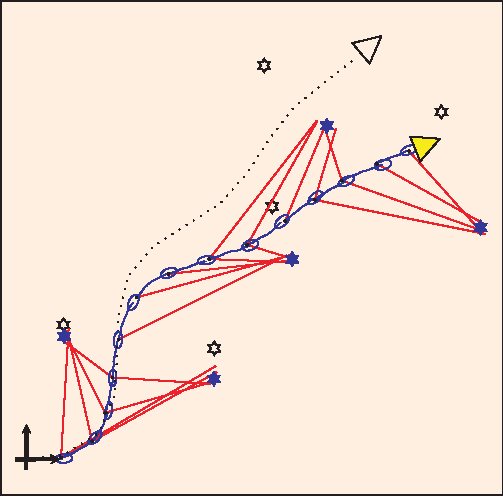
\includegraphics[width=0.6\columnwidth]{imgs/RBPF_trajectory.pdf}
	\end{center}
	\caption{Propojení odhadované trajektorie s pozorovanými landmarky (z [5]).}
	\label{fig:RBPF_trajectory}
\end{figure}

\newpage

\subsection{Graph-based SLAM}
Graph-based SLAM je algoritmus založený na metodě nejmenších čtverců. Jedná se o offline algoritmus rozdělený do dvou částí, front-end a back-end.\\
\indent Metoda nejmenších čtverců je optimalizační metoda počítající s přeurčeným systémem, kdy je známo více rovnic, než je neznámých. Metodu představil na konci 18. století Carl Friedrich Gauss, a jak z názvu vyplývá, snaží se minimalizovat sumu chyb ve čtverci. Chyba je zde definována jako rozdíl odhadovaného stavu k aktuálnímu měření:
\begin{equation}
	\textbf{e}_i(x)=\textbf{z}_i-\textbf{f}_i(x)
\end{equation}  
Jedním z předpokladů pro správný průběh metody je dobrý počáteční odhad stavu. Dále, okolí minima chyby musí být hladké, bez skoků a zubů. V této oblasti se provádí lokální linearizace prvním stupněm Taylorova polynomu. Následně je vypočítána první derivace funkce chyby ve čtverci, která se položí rovna nule. Vyřeší se lineární systém, získá se nový stav, který by měl být lepší, než ten předchozí. Poté se znovu iteruje.
\begin{figure}[!ht]
	\begin{center}
		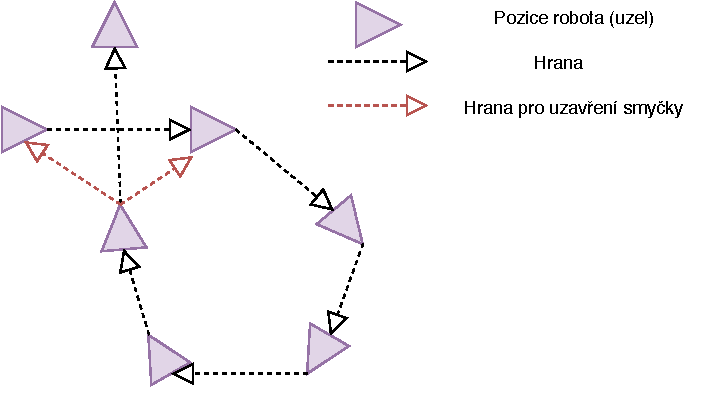
\includegraphics[width=0.5\columnwidth]{imgs/GBS_constrains.pdf}
	\end{center}
	\caption{Propojení uzlů pomocí hran.}
	\label{fig:GBS_constrains}
\end{figure}
\subsubsection{Tvorba pozičního grafu}
Tvorba grafu je první částí metody Graph-based SLAM, tedy část vývojová (front-end). Dochází zde ke tvorbě pozičního grafu, který je zpracováván do mapy. Graf se složen ze dvou složek, a to z uzlů a hran. Uzel zde znázorňuje odhadovanou pozici robota a hrana omezení, které je mezi dvěma uzly. Toto spojení je nejisté a proměnné. Při projetí známým prostředím se vytvářejí hrany mezi uzlem novým a uzly již dříve zaznamenanými, což je využito například při uzavírání smyčky (viz. obrázek \ref{fig:GBS_constrains}).\\
\indent Nové hrany vznikají při splnění jedné ze dvou podmínek. Pokud je zaznamenán přesun robota z pozice $x_i$ do $x_{i+1}$, hrana odpovídá naměřenné odometrii. Druhou možností je zpozorování stejného prostředí. Vzniká tak virtuální měření, ve kterém se porovnají obě tyto pozorování. Na základě rozdílu odhadované pozice při obou měřeních, se umístí nový uzel spojený odpovídající hranou(viz. obrázek \ref{fig:GBS_virtual_measurment}). 

\subsubsection{Optimalizace mapy}
Druhou částí algoritmu Graph-based SLAM je back-end část, která zodpovídá za optimalizaci získaného grafu. Upravuje se zde pozice uzlů tak, aby byl získán stav, který co nejpřesněji vystihuje získaná měření. Po tomto procesu je pak možno utvořit mapu na základě známých pozic.\\
\indent Rovnice pro optimalizaci vychází z metody nejmenších čtverců:
\begin{equation}
	\textbf{x}^*=argmin_{\textbf{x}}\Sigma_{ij}\textbf{e}_{ij}^T(\textbf{x}_i,\textbf{x}_j)\Omega_{ij}\textbf{e}_{ij},
\end{equation}
kde $\textbf{x}^*$ je cílové rozmístění uzlů, chyba $\textbf{e}_{ij}$ vychází z (rovnice nahoře) a $\Omega_{ij}$ je informační matice pro danou hranu. 

\begin{figure}[!ht]
	\begin{center}
		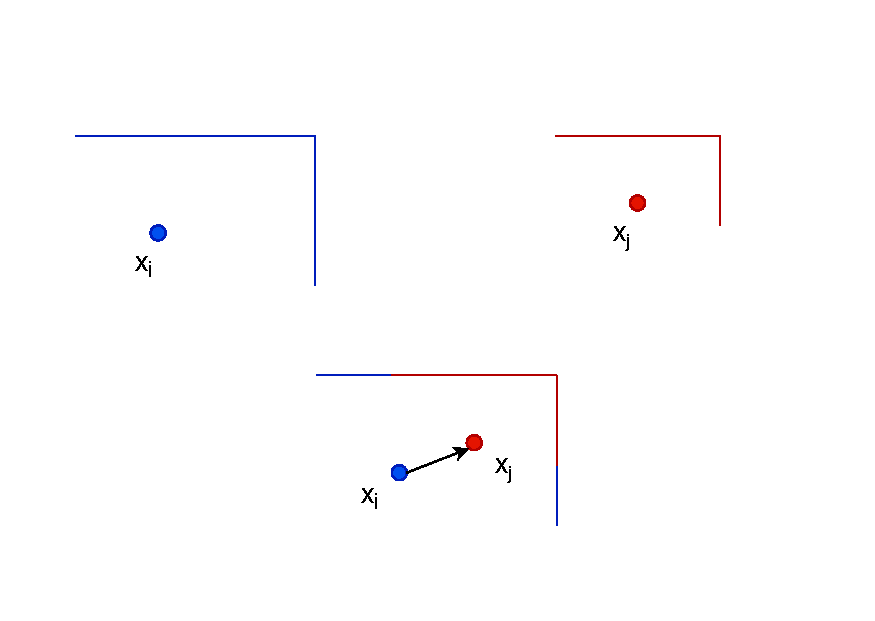
\includegraphics[width=0.6\columnwidth]{imgs/GBS_virtual_measurment.pdf}
	\end{center}
	\caption{Znázornění funkce virtuálního měření.}
	\label{fig:GBS_virtual_measurment}
\end{figure}

\newpage
\subsection{Reprezentace prostředí}
Původně se svět modeloval jen jako soubor landmarků majících svůj určitý tvar, později však, zejména ve venkovním, podvodním a podzemním použití, se ukázala tato metoda jako nevyhovující. Hledaly se tak další metody, které by zlepšily reprezentaci prostředí. Výsledné možnosti jsou popsány v následujících odstavích.

\subsubsection{Mapa z landmarků}
V počátcích vývoje problému SLAM bylo pochopitelně potřeba vymyslet, jak reprezentovat výsledky měření a pozorování. Vznikla tedy metoda, kdy podobu mapy utvářely landmarky samotné. Když je nový landmark zpozorován, je zanesen do mapy a vytvoří se korelace k ostatním, již pozorovaným landmarkům. Odhadovaná pozice robota je také korelovaná vůči všem landmarkům. \\
\indent Opětovným projížděním známého místa korelace mezi landmarky roste a mapa se zpřesňuje. Tím, že jsou všechny landmarky ve vzájemné korelaci, vytváří se pomyslná síť z těchto spojení. Tato metoda může být při správné implementaci tedy velmi přesná. Problémem je však výpočetní náročnost, která kvadraticky roste s přibývajícími landmarky. Pro menší prostředí se tedy metoda využít dá, pro větší je to ale výkonově příliš náročné.

\begin{figure}[!ht]
	\begin{center}
		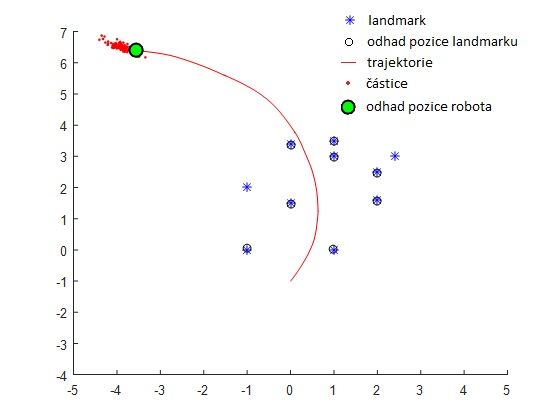
\includegraphics[width=0.7\columnwidth]{imgs/landmark_map.jpg}
	\end{center}
	\caption{Ukázka mapy z landmarků.}
	\label{fig:landmark_map}
\end{figure}
\newpage
\subsubsection{Mřížkové mapy}
Metoda mřížkových map, v originále $Grid$ $maps$, byla představena v 80. letech minulého století. Její základní myšlenkou je diskretizace spojitého prostředí do jednotlivých buněk, přičemž mřížky rozdělující prostor na buňky mají pevnou velikost. Metoda je poměrně náročná na paměť.\\
\indent Důležitým faktorem je zde takzvaná obsazenost, v angličtině $occupancy$. V originále se tedy metoda nazývá $Occupancy$ $Grid$ $Maps$. Pravděpodobnost obsazení každé buňky může nabývat tří hodnot. Při inicializaci je hodnota pravděpodobnosti nastavena na $P(m_i)=0.5$, kdy $m_i$ je daná buňka. Tato počáteční hodnota znamená, že o buňce nemáme žádnou znalost. Poté, co se buňka dostane do dosahu senzoru, nabývá pravěpodobnost obsazenosti již pouze dvou hodnot. $P(m_i)=0$, pokud je buňka neobsazená a $P(m_i)=1$ v případě obsazenosti.\\
\indent Buňky jsou na sobě zcela nezávislé a součinem pravděpodobností obsazení buněk je získáno pravděpodobnostní rozložení mapy:
\begin{equation}
	p(m)=\Pi_ip(m_i)
\end{equation}
Odhad mapy ze senzoru:
\begin{equation}
	p(m|z_{1:t},x_{1:t})=\Pi_ip(m_i|z_{1:t},x_{1:t}),
\end{equation}
kdy $z_{1:t}$ jsou pozorování a $x_{1:t}$ pozice robota.

\begin{figure}[!ht]
	\begin{center}
		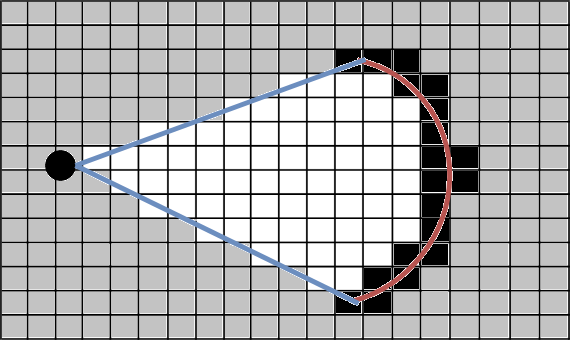
\includegraphics[width=0.7\columnwidth]{imgs/gridmap.png}
	\end{center}
	\caption{Rozložení pravděpodobností mřížkové mapy dle aktuálního měření.}
	\label{fig:grid_map}
\end{figure}
\newpage
\subsubsection{Mračno bodů}
Výše zmíněné metody se vztahují především na práci s daty ve 2D. Pro zahrnutí třetí dimenze do mapy se tak využívají mračna bodů, v originálu $point$ $clouds$. Data se získávají například pomocí kamer, či 3D LIDARů. Výsledné mapy tak vytvářejí komplexnější reprezentaci prostředí, které se skládá z milionů až miliard bodů. Jednotlivé body nesou vždy informaci o své pozici v prostoru, při využití kamery i přímo odpovídající barvu. Barevné rozlišení se dá použít i jinými způsoby. Je možné mít škálu barev, ve které přechází barvy dle zaznamenané výšky. Případně mohou barvy znázorňovat míru pravděpodobnosti, že se daný bod opravdu nachází na odhadované pozici.

\begin{figure}[!ht]
	\begin{center}
		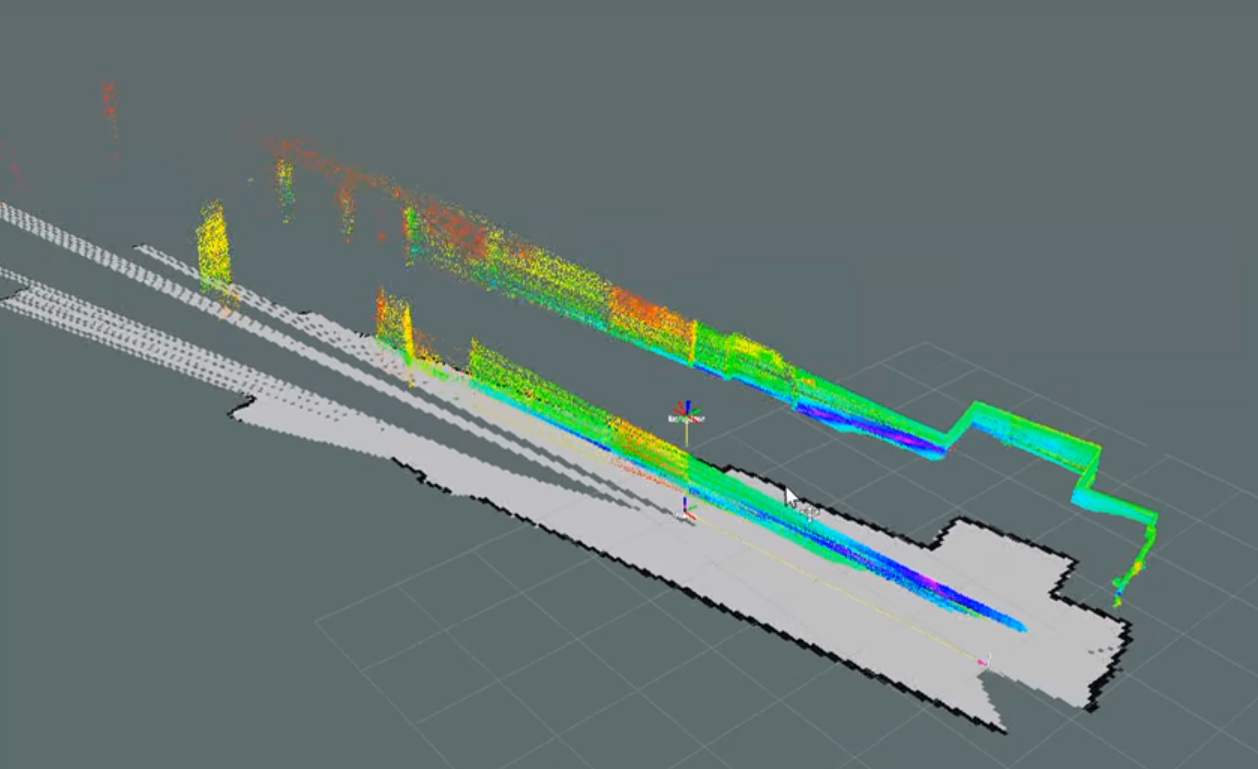
\includegraphics[width=0.7\columnwidth]{imgs/point_cloud.png}
	\end{center}
	\caption{Ukázka mapování pomocí mračna bodů.}
	\label{fig:point_cloud}
\end{figure}

\newpage
\chapter{Systémy SLAM}
V této kapitole jsou popsány vybrané systémy SLAM. Výběr systémů byl proveden na základě největší rozšířenosti. Tímto kritériem byly zvoleny systémy gMapping, Hector SLAM a Google Cartographer. Níže je jednotlivě uvedena doba představení systému, na čem je založen a způsob implementace.

\section{GMapping}
GMapping byl představen v roce 2007 v článku [8]. Tato metoda je založená na implementaci Rao-Blackwellizovaného filtru, kde si každá vytvořená částice nese svoji mapu prostředí. Pro praktické využití je tedy nutné částicový filtr zefektivnit, což bylo úkolem tohoto systému. Jedna možnost je zahrnout přesnost měření do návrhového rozložení, tím je získáno přesné vykreslení částic. Druhou možností, je volba vzorkovací techniky udržující rozumný počet částic. Udržuje se tak přesná mapa a snižuje se riziko vyčerpání částice, což je problém vznikající při převzorkování.\\

\subsection{Mapování pomocí RBPF}
Základním úkolem je odhad posteriorní pravděpodobnosti a tím zisk mapy a trajektorie pohybu. Odhad je prováděn na základě porovnání pozorování a informace z odometrie. Nejprve dochází k odhadu mapy, která je utvářena z porovnání pozorování, poté až trajektorie. Ta je získána z částic, které měly v rozhodovací době největší pravděpodobnost. Každá částice tedy reprezentuje část trajektorie.\\
\indent Pro výběr správné částice je použit částicový filtr, v tomto případěm Sampling Importance Resamplin (SIR), který při mapování postupně zpracovává data ze senzoru, poté odometrii a aktualizuje sadu vzorků reprezentující posteriorní pravděpodobnost, která zahrnuje informace o mapě a trajektorii. \\
\indent Nejprve se získají nové částice. To je provedeno odběrem vzorků z předchozí generace návrhového rozložení. V dalším kroce je částicím nastavena vážená důležitost, aby cílové rozložení nebylo rovno tomu navrhovanému. Poté dochází k převzorkování, kdy jsou částice přepisovány úměrně jejich váženým důležitostem. Nakonec se odhaduje podoba mapy, kdy je pro každou částici, na základě trajektorie vzorku a historie pozorování, mapa vypočítána.

\begin{figure}[!ht]
	\begin{center}
		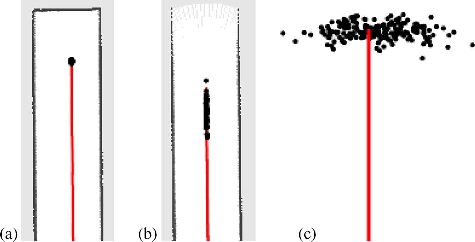
\includegraphics[width=0.7\columnwidth]{imgs/gmapping_particles.pdf}
	\end{center}
	\caption{Rozložení částic dle typu prostředí.\\
	a) konec chodby, b) cesta chodbou, c) otevřený prostor (z [9])}
	\label{fig:gmapping_particles}
\end{figure}


\subsection{Vylepšené návrhy a adaptivní převzorkování}
Pro zisk nové generace částic je třeba vykreslení vzorků z návrhového rozložení, kde platí úměra, čím lepší návrh, tím lepší výsledek. Kdyby byl návrh rovný cílovému rozložení, částice by měly stejnou váženou důležitost a převzorkování by nebylo třeba. \\
\indent Návrhové rozložení typicky odpovídá odometrickému pohybovému modelu, který však není optimální a to zejména, pokud je senzor výrazně přesnější než odhad pozice. Využívá se také vyhlazování pravděpodobnostní funkce, což zabraňuje částicím v okolí významné oblasti, aby vážené důležitosti příliš poklesly. Následkem je ale zkreslení mapy. To se však dá vyřešit zahrnutím posledního pozorování do generování nových vzorků. Díky tomu se systém zaměřuje na vzorkování ve významné oblasti pravděpodobnosti pozorování.\\
\indent Zlepšením návrhu se objevuje možnost získávat pro každou částici zvlášť její parametry Gaussiánského návrhu a snižuje se také neurčitost výsledných hustot pravěpodobností. Porovnání pozorování má funkci maximalizace pravděpodobnosti pozorování, tvorby mapy a počáteční odhad pozice robota. Pokud je pravděpodobnostní funkce vícerežimová, například při uzavírání smyčky, porovnáním se vrací nejbližší lokální maximum pro každou částici. To může způsobit vynechání některých maxim v pavděpodobnostní funkci.\\
\indent Převzorkování je velice důležitým aspektem určujícím výkon částicového filtru. Dochází k nahrazování vzorků s nízkou vahou. Je to nezbytný proces, neboť je potřeba konečného počtu částic pro aproximaci cílového rozložení. Může však odstranit dobré vzorky a ochudit tak částice, je proto důležité mít pro převzorkování vhodné rozhodovací kritérium a provádět ho ve správný čas. 
\begin{equation}
	N_{eff}=\frac{1}{\varSigma_{i-1}^N(w^{(i)})^2},
\end{equation} 
$w^{(i)}$ je zde normalizovaná váha částice $i$ a $N_{eff}$ jsou vzorky z cílového rozložení, které mají stejné váhové důležitosti. Pokud dochází ke zhoršení aproximace cílového rozložení, nastává větší odchylka vážených důležitostí.\\
Základní nastavení převzorkování je následující:
\begin{equation}
	N_{eff} < N/2,
\end{equation}
kde $N$ je počet částic. Tím dochází k výrazné redukci možnosti nahrazení dobrých částic a počtu převzorkování, které se vykonává pouze pokud je třeba.\\
\indent Algoritmus probíhá následovně. Dojde k zisku odhadu pozice, který je reprezentovaný danou částicí. Odhad je získán z předchozí pozice částice a odometrického měření od poslední aktualizace. Na základě mapy je provedeno porovnání pozorování z místa úvodního odhadu pozice, kdy se vyhledává pouze v okolí tohoto bodu. V případě selhání se pozice a váhy počítají dle pohybového modelu a následující dva kroky jsou přeskočeny. Prvním z nich je vybrání sady vzorků v okolí dané pozice, vypočítání průměrů a kovarianční matice návrhu pomocí bodového ohodnocení cílového rozložení v pozici vzorku. Druhým, potenciálně přeskočeným krokem, je zakreslení nové pozice částice z Gaussovské aproximace podle zlepšeného návrhového rozložení. Dále, a to již vždy, dojde k aktualizaci vážených důležitostí a, podle zakreslené pozice a pozorování, je aktualizována i mapa částice. 
 
\newpage

\section{Hector SLAM}

Hector SLAM je systém představený v roce 2011 v práci [9]. Jeho hlavním znakem je rychlost a nízké výpočetní nároky oproti ostatním dvěma metodám, které jsou v této práci rozebírány. Je vhodný pro implementaci v menších autonomních systémech, pro rychlý pohyb terénem a nehodí se pro uzavírání velkých smyček.\\
\indent Vnitřní skladba systému je ze tří hlavních částí, a to 2D SLAM, běžící jako soft real time, 3D navigace, která je hard real time a inerciální jednotka (IMU). Hector SLAM je front-end SLAM, což znamená, že dochází k odhadu stavu robota v reálném čase a nedochází ke zpětné optimalizaci mapy.\\
\indent Daný systém se musí převézt z 3DOF přidáním naklonění a rotace na 6DOF, kdy navigační filtr spojí měření z IMU a dalších senzorů. Tím dojde k získání 3D řešení. 2D SLAM poté poskytuje informaci o poloze v prostoru. Oba odhady se aktualizují nezávisle na sobě a jsou propojeny jen velmi málo.\\
\indent Kvůli znatelnému posunu odhadů integrované pozice a rychlosti, který je způsoben šumem v senzorech, jsou do systému zahrnuty další informace. Jedná se například o porovnávání snímků, snímání magnetického pole, senzor barometrického tlaku a nebo měření rychlosti kol.

Pohyb robota je popsán:
\begin{equation}
	\dot{\Omega}=E_\Omega.\omega
\end{equation}
\begin{equation}
	\dot{p}=v\\
\end{equation}
\begin{equation}
	\dot{v}=R_\Omega.a+g,
\end{equation}\\
kde $\Omega=(\phi,\theta,\psi)^T$ je informace o otáčení, stoupání a natočení. Vektor $x=(\Omega^T p^T v^T)^T$ reprezentuje 3D stav, $p,v$ jsou pozice a rychlost platformy v navigačním rámci. Vektor $u=(\omega^T a^T)^T$ je vstupní vektor pro inerciální měření, $\omega=(\omega_x,\omega_y,\omega_z)^T$ je úhlová rychlost a $a=(a_x,a_y,a_z)^T$ je zrychlení. $R_\Omega$ je pak matice směrových cosinů, $E_\Omega$ je mapování natočení těla na deriváty Eulerova úhlu a $g$ je vektor gravitace.\\

\subsection{2D SLAM}
Jako reprezentace prostředí je zde vybrána metoda mřížkových map. Odhadovaná pozice robota slouží pro transformaci pozorování na lokální souřadnicový rámec. Odhadovanou orientací a přidruženými hodnotami je z pozorování vytvořeno mračno bodů, které je předzpracováno pro odstranění odlehlých bodů. Filtrace probíhá pouze na základě souřadnic koncového bodu, kdy jsou pro porovnávání pozorování použity pouze koncové body v rámci skenovací roviny.\\
\indent Jak již bylo poznamenáno, je zde použita struktura mřížkových map, to vede k omezení přesnosti a neumožnění přímého výpočtu interpolovaných hodnot a derivátů. Pro oba odhady se tedy využívá interpolační schéma, díky kterému tato možnost je. Souřadnice, které se potřebují nahradit, se aproximují pomocí čtyř nejbližších integerových souřadnic. \\
\indent Laserové skenery jsou již velice přesná zařízení, jejich měření zatěžuje minimální šum a snímky se dají vytvářet s vysokou frekvencí. Měření pomocí laseru je tedy mnohem přesnější než to odometrické, což je jeden z důvodu, proč je odometrie v tomto systému zcela vynechána. Při zarovnávání snímků s již známou mapou není potřeba hledat žádná spojení mezi koncovými body, ale dochází k porovnávání s předchozími skeny.  

Hledání transformace pro nejlepší sladění skenu s mapou:
\begin{equation}
	\xi^*=argmin_\xi\Sigma_{i=1}^n[1-M(S_i(\xi))]^2
\end{equation}
$M(P_m)$ je zde hodnota obsazenosti a $S_i(\xi)$ jsou souřadnice koncového bodu $s_i=(s_{i,x},s_{i,y})^T$, přičemž $\xi$ jsou souřadnice robota.\\
 
Optimalizace chyby měření: 
\begin{equation}
	\Sigma_{i=1}^n[1-M(S_i(\xi+\Delta\xi))]^2\rightarrow 0,
\end{equation}
kde $\Delta\xi$ je odhad $\xi$.\\
\indent Při tvorbě mapy dochází často k nalezení pouze lokálního minima, reprezentací mapy pomocí více rozlišení se tak toto riziko znatelně redukuje. Utváří se mřížkové mapy, kdy každá další má poloviční rozlišení, než ta předchozí. Je tak uloženo více map, které se součastně aktualizují podle odhadu aktuální pozice. Díky tomuto přístupu jsou mapy konzistentní a nepotřebují převzorkování. Zarovnávání pozorování probíhá pouze na mapě s nejvyšším rozlišením a tento odhad je pak použit pro ostatní mapy. Mapy s nízkým rozlišením jsou tedy v podstatě dostupné okamžitě, a lze je hned využít pro odhad trasy. 

\subsection{Odhad 3D stavu}
Pro odhad úplného 6D stavu (3D stav + informace o naklonění z gyroskopů a informace z akcelerometrů) slouží navigační filtr běžící v reálném čase. Filtr je asynchronně aktualizován při příchodu odhadované pozice z porovnání pozorování nebo jiných informací ze senzorů. Filtr je implementován ve formě EKF, jedná se tedy o nelineární filtr a jako jeho známé vstupy se berou inerciální měření. Rychlost a pozice je získávána integrací zrychlení. Aby se zabránilo nezávislému růstu odhadu stavu při nepřítomnosti měření, dochází k aktualizaci pseudo-nulové rychlosti, která se spouští při dosažení odchylky určité prahové hodnoty a zajišťuje tak stabilitu systému.\\

\newpage

\section{Catographer}

Systém Cartographer je vyvíjen společností Google a aktuální verze implementace byla publikována v roce 2012 [10]. Jedná se o implementaci Graph-Based SLAM. Je vhodný pro tvorbu rozsáhlých map a zisk optimalizovaných výsledků v reálném čase. \\
\indent Cartographer vytváří v reálném čase 2D mřížkovou mapu. Submapy se vkládají na odhadované místo a daná submapa se porovnává vůči poslední zaznamenané. Dochází tedy k hromadění globální chyby z odhadu pozice. Systém neobsahuje žádný částicový filtr a to z důvodu snížení hardwarových nároků na běh algoritmu.\\
\indent Submapa se po pořízení již dále nijak nepřepisuje a je zařazena mezi ostatní k porovnávání na uzavření smyčky. Pokud dojde k blízkému odhadu pozice a zároveň dostatečné shodě snímků, přidá se omezení uzavření smyčky do optimalizačního problému, čímž je odhad pozice. Odhad se aktualizuje po několika vteřinách a uzavření smyčky je tedy okamžitě viditelné.\\
\indent Rozlišují se dva možné přístupy, lokální a globální, v obou případech se jedná o optimalizaci pozice, přičemž pozice se zkládá z hodnoty na ose $x$, z hodnoty na ose $y$ a z natočení robota. V systému je také obsažená jednotka IMU, která slouží k odhadu směru gravitace, což má využití při pohybu na nerovné ploše.\\

\subsection{Lokální 2D SLAM}
\indent Skeny prostředí se iterativně zarovnávají se snímky již obsaženými v submapě. Submapa je tedy v postatě zachycení kousku světa, které je složené z pár skenů. Lokální chyba, vznikající při její tvorbě, je poté odstraněna v globálním přístupu. Pro každý bod mřížky je definován odpovídající pixel skládající se ze všech pixelů nejblíže danému bodu.\\
\indent Při přidání skenu do pravděpodobnostní mřížky je počítána množina zasažených bodů mřížky a bodů minutých. Při zásahu se nejbližší bod mřížky vloží do množiny zásahů. Při nezaznamenání překážky jsou vloženy do množiny minutí všechny body odpovídající dráze laserového paprsku. Dosud nepozorované body mřížky mají přiřazenou pravděpodobnost minutí či zásahu, podle toho, jestli se v jedné z těchto množin vyskytují. Již pozorovaným bodům se pak aktualizují pravděpodobnosti minutí a zásahu.\\
\indent Před vložením skenu do submapy se ještě využívá Ceres scan matching, který optimalizuje pozici skenu vůči submapě. Jedná se o maximalizaci pravděpodobnosti výskytu v dané oblasti.  

\begin{equation}
argmin_\xi\Sigma^K_{k=1}(1-M(T_{\xi}h_k))
\end{equation}

$H$ je zde informace o bodech skenu, $M$ je pravděpodobnostní mřížka, $\xi$ je pozice snímání skenu a $T_{\xi}$ je pozice skenu vůči submapě. Dochází k transormaci, kdy body skenu se transformují do submapy.

\begin{figure}[!ht]
	\begin{center}
		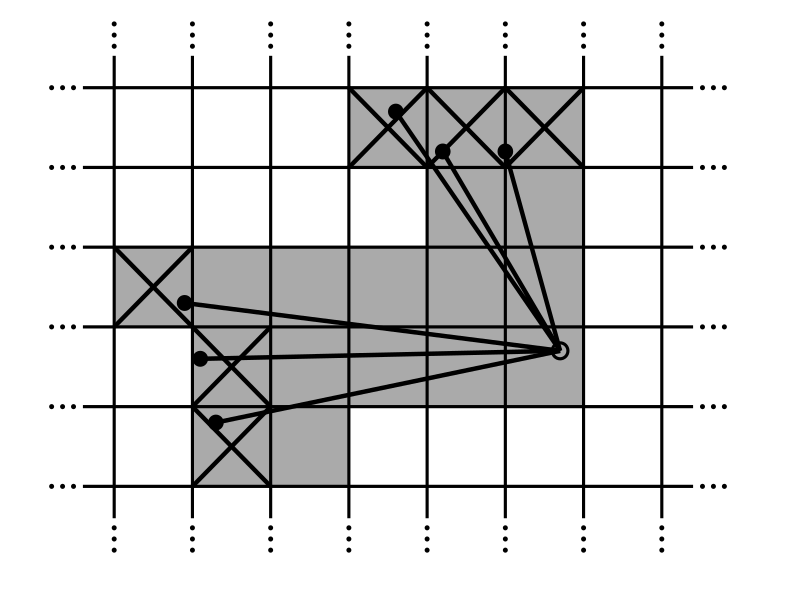
\includegraphics[width=0.7\columnwidth]{imgs/cartographer.png}
	\end{center}
	\caption{Vizualizace zasažení a minutí bodů v mřížce (z [10])}
	\label{fig:cartographer}
\end{figure}

\subsection{Globální 2D SLAM}
Daný systém pracuje v oblasti submap s porovnáváním scan-to-scan, hromadí se v něm tedy lokální chyby. Pár snímků za sebou má však vůči sobě chybu minimální. Relativní pozice skenů se ukládají a v případě, že se submapa nezmění, všechny další páry ze skenů a submapy se předkládají k porovnávání pro uzavření smyčky. To vše běží na pozadí a pokud je nalezena shoda, dojde k uložení relativní pozice mezi optimalizační problémy.\\
\indent Optimalizační problém je problém nelineárních nejmenších čtverců. Díky tomu se můžou jednoduše přidávat zbytky pro zohledňování dalších dat. Jednou za pár sekund je, pro optimalizaci pozice skenu vůči daným omezením, spuštěn Ceres scan matching. Omezeními jsou myšlena relativní pozice $\xi_{ij}$ a kovarianční matice $\Sigma_{ij}$.
\begin{equation}
argmin_{\Xi^m,\Xi^s}\frac{1}{2}\Sigma_{ij}\rho(E^2(\xi_i^m,\xi_j^s,\Sigma_{ij},\xi_{ij})),
\end{equation}\\
kde $\rho$ je ztrátová funkce, například tedy Hubertova ztráta. Jedná se o snížení vlivu odlehlých hodnot, které přidávají nesprávná omezení do optimalizačního problému.\\
\indent Při uzavírání smyčky se vyžívá také branch-and-bound scan matching, což se dá přeložit jako porovnávání větví a mezí. Zde se metoda zaměřuje na přesnou shodu pixelů. Podmnožiny možností jsou popsány jako uzly stromu, kdy kořenový uzel obsahuje všechna možné možnosti $W$. Potomci uzlu dohromady utváří stejný soubor možností, jako samotný rodičovský uzel. Listy jsou brány jako singlety, odpovídají jedinému proveditelnému řešení. Tento přístup dává stejné řešení jako ten předchozí, dokud je hodnota $score(c)$ vnitřních uzlů horní mezní skóre jeho prvků. Neexistuje tedy žádné řešení, než to doposud známé.

\begin{equation}
\xi^*=argmax_{(\xi\epsilon W)}\Sigma_{k=1}^KM_{nearest}(T_{\xi}h_k)
\end{equation}\\
$W$ je zde vyhledávací okno a $M_{nearest}$ je rozšíření pravděpodobnostní mřížky $M$ na všechny $R^2$ zaokrouhlením argumentů do nejbližšího bodu mřížky. Rozšířená hodnota bodu mřížky ukazuje na odpovídající pixel.\\
\indent Výběr uzlů probíhá prohledáváním do hloubky. Efektivnost algoritmu hodně závisí na podobě stromu, zda-li má pro výpočet dobrou horní mez a dobré aktuální řešení. Důležitým termínem je zde prahová hodnota skóre. Jedná se o hodnotu, pod níž není v zájmu jít a řešení je tedy nevyhovující. Díky tomu se nepřidávají špatné shody jako omezení pro uzavírání smyčky. Pro rychlost algoritmu je důležité rozhodování o průchodu stromem. Pro každého potomka je vypočítána horní hranice skóre a je vybrán ten nejslibnější, což je uzel s největším mezním počtem.\\
\indent Každý z uzlů je popsán pomocí pole integerů: 
\begin{equation}
c=(c_x,c_y,c_\Theta,c_h)\epsilon Z^4,
\end{equation}
kde $c_h$ je výška uzlu. Pokud $c_h=0$, uzel je list.\\
\indent Horní meze jsou pak počítány přes vnitřní uzly: 
\begin{equation}
score(c)=\Sigma_{k=1}^Kmax_{(j\epsilon \bar{W})}M_{nearest}(T_{\xi_j}h_k)
\end{equation}

\newpage

\chapter{Experimentální měření}
Pro testování všech výše zmíněných systémů bylo využito frameworku $Robot$ $Operating$ $System$ (ROS). V této části práce je tedy popsána jeho funkčnost a využití. Dále je zde porovnání implementací SLAM, jak na simulačních datech, tak i na datech reálných. Porovnání je provedeno výpočtem chyb v trajektoriích jízdy a v případě nekonvergence systému rozebráním situace, proč k danému problému došlo.

\section{Robot Operating System}
Robot operating system, zkráceně ROS, je operační systém určený pro ovládání robotů. Poskytuje vše očekávané od operačního systému, jako je například abstrakce hardwaru, nízkoúrovňové ovládání, komunikace mezi procesy a mnoho dalších funkcí. Obsahuje také nástroje a knihovny pro vytváření, získávání, psaní a spouštění kódu na více zařízeních. ROS prozatím běží pouze na platformách založených na Unixu. Software je testovaný především na systémech s Ubuntu nebo Mac OS X, přičemž s Windows není zatím kompatibilní.\\
\indent Při běhu je komunikační infrastrukturou ROSu vytvářena síť volně propojených procesů, které mohou běžet na více zařízeních. Implementováno je zde několik možných komunikačních stylů. Přes služby je to synchronní komunikace RPC ($Remote$ $Procedure$ $Call$ = vzdálené volání procedur). Je to jedna z nejstarších metod pro komunikaci programů na dálku. Obsahuje mechanismus umožňující volat z programu funkce ze vzdáleného počítače. Dalším obsaženým stylem komunikace, je asynchronní streamování dat, které běží přes topiky. Posledním je ukládání dat na $Parameter$ $Server$, což je sdílený víceúrovňový slovník, který je přístupný prostřednictvím síťových rozhranní API. Procesy, označované jako uzly ($nodes$, nody), využívají tento server k ukládání a načítání dat za běhu.\\
\indent Existuje celá řada softwarových platforem pro roboty a je těžké porovnávat, která z nich je ta nejlepší. ROS je open source systém, hlavní jeho snahou je znovuvyužitelnost napsaného kódu a multiplatformní provozuschopnost, což z něj činí nejrozšířenější systém pro roboty. Celý rámec je složený z distribuovaných procesů, nodů. Nody jsou individuáně spustitelné soubory, které se ze běhu volně propojují do peer-to-peer sítě, mohou být seskupeny do balíků a být tak jednoduše sdíleny.\\
\indent Jednou z dalších snah systému ROS je co největší hubenost. Nedochází k zabalení metody main() a tím může být kód využit i jinými frameworky. ROS je tak snadné integrovat s dalšími robotickými softwarovými frameworky, jako je například OpenRAVE nebo OROCOS. Dalším důležitým rysem je jazyková nezávislost, kdy je možné plně využívat jazyků Python, C++ a Lisp. Dále, zatím experimentálně, je možné používat určité knihovny z jazyků Java a Lua. Neméně důležitými vlatnostmi jsou také škálovatelnost, což je pro velké runtime systémy vlastnost velmi užitečná a snadné testování pomocí vestavěné jednotky $rostest$.\\
\indent Ros se skládá ze tří úrovní pojmů. První úrovní je souborový systém, další je výpočetní graf a poslední je komunitní úroveň.\\

\subsection{Souborový systém}
Na úrovni souborového systému jsou v ROSu myšleny všechny prostředky, se kterými se pracuje na pevném disku. Jedná se o balíčky ($Pakages$), metabalíčky ($Metapackages$), $Package$ $Manifests$, repozitáře, typy zpráv a typy služeb.\\
\indent Balíčky jsou základní stavební jednotkou softwaru ROS. Jedná se o nejnižší strukturu umožňující tvorbu programu. Balíčky mohou obsahovat $ROS$ $runtime$ procesy, dále knihovny závislé na ROSu, datové sady, konfigurační soubory a mnoho dalšího, co lze užitečně zahrnout do jednoho souboru.\\
\indent Metabalíčky se již nachází výše, je to specializovaný balíček, který slouží k reprezentaci skupiny souvisejících balíčků. Nejčastější jejich využití je držení zpětné kompatibility pro zásobníky ($Stacks$), které prošly konverzí přes $rosbuild$. Zásobníky jsou též kolekce balíčků, které seskupují určité funkce, například $navigation$ $stack$, jenž na základě informací ze senzorů dává příkazy pro další navigaci robota v prostředí. $Package$ $Manifest$, package.xml, poskytuje metadata o daném balíčku. Jsou v něm obsažené informace jako název, verze, popis, licenční informace, závislosti a další.\\
\indent Repozitář je opět souhrn balíčků (může však obsahovat pouze jeden balíček), které sdílejí společný systém kontroly stejné verze ($Version$ $Controlling$ $System$, VCS). Balíčky tak mohou být společně uvolněny užitím nástoje $catkin$. Repozitáře často mapují převedené zásobníky přes $rosbuild$.\\
\indent Typy zpráv a typy služeb pak již definují typy, které se smějí v ROS využívat. Pro typy zpráv je cesta k souboru $my\_package/msg/MyMessageType.msg$ a obsahuje datové struktury pro posílané zprávy. Definice typů služeb se nachází na adrese $my\_package/srv/MyServiceType.srv$ a definuje datové struktury požadavků a odpovědí.\\

\subsection{Výpočetní graf}
Výpočetní graf se skládá z jednotlivých procesů zpracovávajících společně sdílená data a dohromady vytvářejících peer-to-peer síť. Základními pojmy pro výpočetní graf jsou nody ($nodes$), $Master$, $Parameter$ $Server$, zprávy ($messages$), topiky ($topics$), služby a bagy. Všechny pojmy jsou implementovány v repozitáři pro komunikaci $ros\_comm$.\\
\indent Nody, neboli uzly, jsou procesy obstarávající výpočty. Řídicí systémy pro robota obsahují často mnoho uzlů. Pro ROS je typická snaha o co největší modularitu, každý uzel má tak jednu svoji úlohu, například zpracování laserového senzoru. Uzly jsou nejčastěji psány pomocí knihoven $roscpp$ nebo $rospy$, kde písmena za $ros$ znamenají, zda-li se jedná o implementaci jazyka C++ nebo Python.\\
\indent $Master$ zde zajišťuje registraci jmen a vyhledávání ve výpočetním grafu. Uzly s $Masterem$ komunikují a oznamují mu své registrační údaje, bez něj by se tedy uzly navzájem nemohly najít a vyměňovat si zprávy. Při změně registračních údajů provede $Master$ zpětné volání uzlů, tím je zajištěno dynamické vytváření spojení mezi uzly. Blízce související termín je $Parameter$ $Server$, který je součástí $Mastera$ a umožňuje ukládání dat do centrálního umístění.\\
\indent Zprávy jsou informace posílané mezi uzly. Jsou tvořeny datovými typy jako je integer, float, boolean a tak dále a nebo ve formě pole obsahujících tyto primitivní typy.\\
\indent Topik je název sloužící k identifikaci obsahu, kterým je určitá zpráva. Pokud uzel vyžaduje určitý typ dat, začne odebírat data z příslušného topiku. Pokud chce uzel data do topiku odesílat, publikuje do něj danou zprávu. Do jednoho topiku může zapisovat i číst z něj zároveň více uzlů a jeden uzel může odebírat a publikovat do více topiků. Uzly, ať publikující, či odebírající, nejsou si vědomy ostatních účastníků u daného topiku.\\
\indent Komunikační model typu publikující/odběratel je vhodný pro posílání zpráv. Pro distribuované systémy, které využívají interakce typu žádost/odpověď, je to však nevyhovující. Tato interakce se tedy provádí pomocí služeb, které jsou definovány dvojicí struktur. Jedna pro žádost a druhá pro odpověď. Například uzel nabízí určitou službu pod jménem a klient této služby využívá zasláním požadavku, kdy poté čeká na odpověď.\\
\indent Posledním pojmem jsou zde bagy, v originálu $Bags$, které slouží k uložení a přehrávání dat z topiků. Jedná se o důležitý mechanismus skladování dat, který je nezbytný pro vývoj a testování algoritmů.\\
\indent Pro ROS jsou velmi důležitá pojmenování. Jména jsou primárním prostředkem pro vybudování velkého a složitého systému. Každy uzel, topik, služba nebo parametr má svůj název. Všechny klientské knihovny podporují přemapování názvu z příkazového řádku, běžící programy tak mohou být za běhu překonfigurovány, aby fungovaly i odlišné topologii výpočetního grafu.\\

\subsection{Komunitní úroveň}
Jedná se o zdroje, které umožňují různým skupinám vývojářů, vyměňovat si software a znalosti. Spadají sem distribuce, což jsou kolekce verzovaných stacků, které lze nainstalovat. Mají dost podobnou úlohu jako distribuce Linuxu, usnadňují tedy instalaci kolekce softwaru a následné udržování konzistentní verze. Dále sem patří repozitáře, kdy různé instituce mohou vyvíjet své vlastní softwarové komponenty robota a sdílet je tak pomocí federované sítě úložišť. Velmi důležitým zdrojem je $The$ $ROS$ $Wiki$, což je hlavní fórum pro dokumentaci informací o ROSu. Kdokoliv přihlášený na svůj účet tak může přidávat nové, či upravovat a aktualizovat již vzniklé dokumentace, psát návody a mnoho dalších věcí užitečných pro komunitu.

\newpage

\section{Zisk dat k porovnání}
Data potřebná pro porovnávání se dají získat prostřdednictvím internetu. Existují veřejně přístupné nahrané datasety z MIT, Deutsche Museum a řady dalších míst. Pro vyzkoušení systémů na velkých datech je tedy daná možnost také využita. Pro porovnání implementací jsou ale převážně použity datasety získané jak ze simulace v ROS, tak i reálná data naměřená robotem $Dagu$ $Wild$ $Thumper$ $6WD$. Získání datasetu je pro porovnání implementací zásadním faktorem. Systémy SLAM mohou samozřejmě jednotlivě běžet na aktuálně simulovaných datech, pro správné porovnání jsou však potřebná data totožná.\\ 
\indent Datasety jsou v ROS ukládány ve formátu $bag$, kde se jsou nahrány vybrané topiky. Pro každou porovnávanou implementaci byly vytvořeny $launch$ soubory, které při zavolání spouštějí uvedené uzly se specifikovaným nastavením. Soubory $launch$ byly pro všechny systémy nastaveny tak, aby potřebovaly informaci o měření z LIDARu, odometrickou informaci a transformaci přepočítávající pozici robota. Tyto tři typy informací stačí při spuštění dané metody k vytvoření mapy a všeho k tomu přidruženého. Pro porovnání trajektorií je potřeba uložit ještě informaci o přesné pozici robota, neboli $ground$ $truth$. V nahraných souborech $bag$ se tedy nachází pouze tyto zmíněné čtyři informace. Výjimkou jsou data získaná robotem $Wild$ $Thumper$. $Ground$ $truth$ by zde měla vycházet z odometrie kol, tudíž o informaci méně. Odometrie z kol robota je však natolik nepřesná, že se pro účely porovnávání nedá využít. Tato nepřesnost samozřejmě zhoršuje provedení metod, které odometrii využívají (Cartographer, gMapping), podrobnější popis dané problematiky se nachází u vyhodnocení daného typu naměřených dat.

\subsection{Simulace v ROS}
Pro zisk dat pomocí simulace jsou v systému ROS implementovány dva hlavní simulátory. Prvním z nich je $Gazebo$. Jedná se o nástroj určený pro simulaci ve 3D, stále prochází vývojem a je nejpoužívanějším simulátorem v ROS. Pro dané účely má však zbytečně veliké množství nastavení. Byl zvolen tedy nástroj $Stage$, který je starší, má méně funkcí, má ale také menší výkonostní nároky a pro simulaci robota s 2D LIDARem je naprosto vyhovující.\\
\indent Simulační prostředí je rozloženo do tří souborů. Dva s příponou $inc$, kdy první obsahuje informace pro načtení mapy. Jsou zde obsaženy informace o velikosti, frekvenci obnovování, výšce překážek v ose $z$ a různá boolean nastavení. V druhém $inc$ souboru se pak nachází informace o simulačním robotovi. Byla zvolena trojúhleníková platforma, na které se nachází malý čtvercový blok simulující LIDAR. Je zde obsaženo i jeho nastavení, jako je počet paprsků, úhel rozsahu a velikost dosahu. Posledním konfiguračním souborem je soubor $wolrd$, ve kterém se nachází nastavení velikosti okna a načtení obou souborů $inc$. Při načítání souboru s nastevením mapy je zde definován obrázek obsahující mapu a s načítáním souboru o robotovi se definuje jeho pozice v prostoru.\\
\indent Pro nahrání dat poté stačí příkazem
\begin{center}
	\texttt{rosrun stage\_ros stageros file.world}
\end{center}
spustit simulaci a pomocí některého z navigačních balíčků s robotem v mapě jezdit. Pro navigaci byla zvolena knihovna $teleop\_twist\_keyboard$, která umožňuje navigaci robota pomocí klávesnice.

\begin{figure}[!ht]
	\begin{center}
		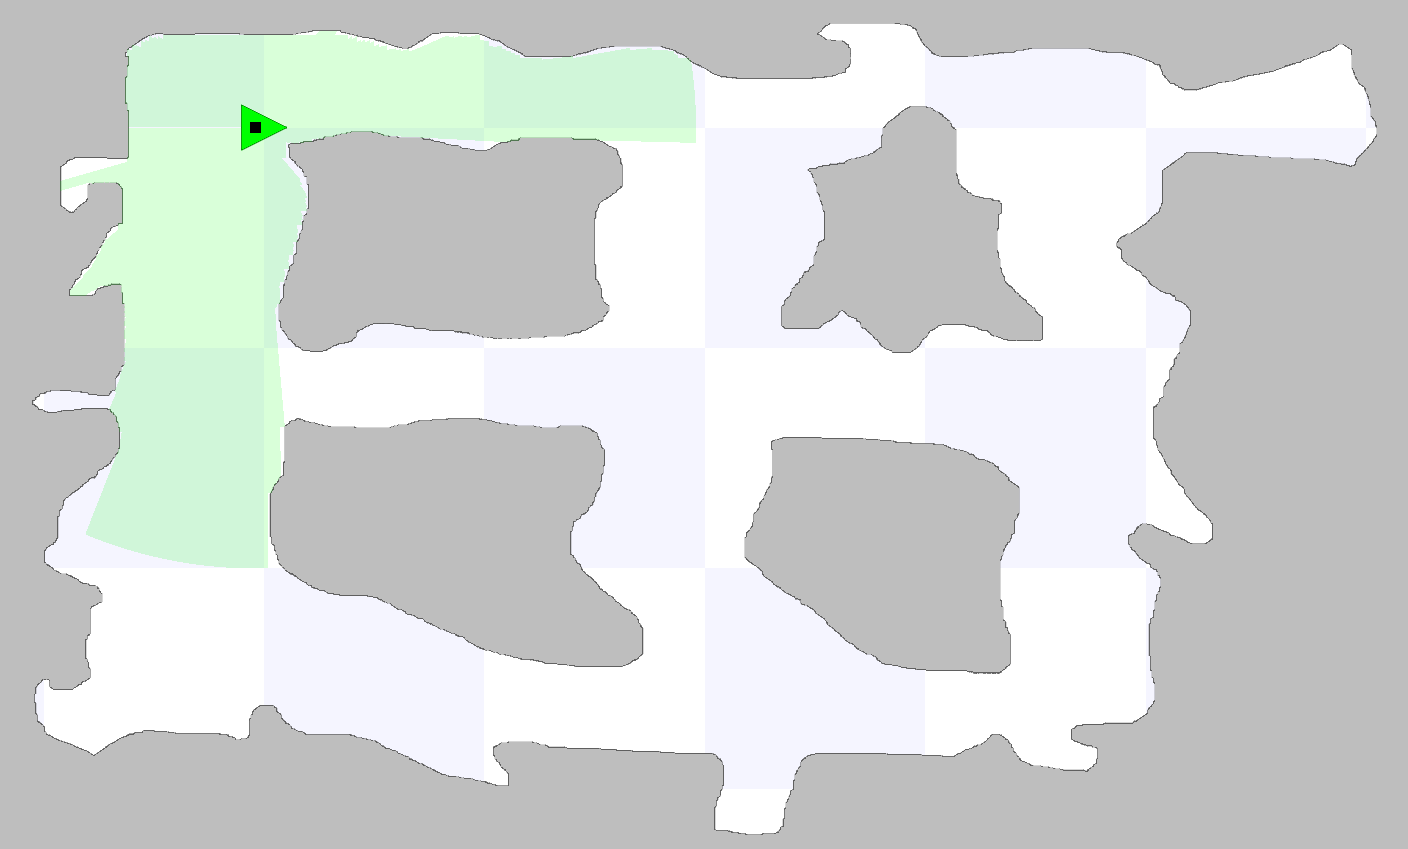
\includegraphics[width=0.7\columnwidth]{imgs/stage.png}
	\end{center}
	\caption{Prostředí Stage}
	\label{fig:stage}
\end{figure}



\subsection{Nahrání reálných dat}
K nahrání reálného datasetu byl k dispozici robot $Wild$ $Thumper$ $6WD$. Jedná se o robota s pohonem šesti kol. Hliníkové tělo má v sobě s rozestupem jednoho centimetru díry, díky kterým se na něj dají jednoduše přidělat další součástky. \\
\indent Pro řízení kol je využito Arduino, pro zpracování dat a komunikaci je zde superpočítač od společnosti NVIDIA, jehož označení je Jetson TX2 a velikost 50 x 87 milimetrů. Výpočetní výkon zajišťuje osmijádrový procesor s architekturou jádra ARMv8. Velikost operační paměti má 8 GB a úložiště 32 GB. Pro komunikaci je zde rozhraní Wi-Fi 802.11ac a Bluetooth 4.1. Jako měřící senzor je zde využit LIDAR $Hokuyo$ $URG-04LX-UG01$ s detekovatelným rozsahem od dvou centimetrů do 5,6 metru. Daný sezor má rozsah snímání 240$^o$ s úhlovým rozlišením 0,36$^o$. Obnovovací frekvence je 100 milisekund a uvedená přesnost je 30 milimetrů.\\
\indent Pro pohyb robota v prostoru byla využita možnost připojení bezdrátového ovladače $Xbox$ $One$ $Wireless$ $Controller$. Přesto, že robot díky integrovanému počítači od NVIDIA má velmi vysoký výkon, tyto prostředky byly nevyužity a data byla při běhu programu posílána rovnou do počítače, kde se následně ukládala do souboru $bag$. Spojení bylo zprostředkováno Wi-Fi routerem $Ubiquiti$ $AirCube$ $AC$, který musí být připojen ethernetovým kabelem k danému počítači. Tento druh propojení má své jisté výhody i nevýhody. Výhodou je bezproblémový přenos, který při připojení robota rovnou na univerzitní Wi-Fi nebyl zdaleka pravidlem. Nevýhodou tohoto řešení je dosah, který je limitován, stejně tak jako je tomu běžně u vysílačů Wi-Fi signálu. Pro dané účely to však nakonec nebyl problém a vhodným umístěním routeru byla možnost naměřit data na dostatečném prostoru. 

\begin{figure}[!ht]
	\begin{center}
		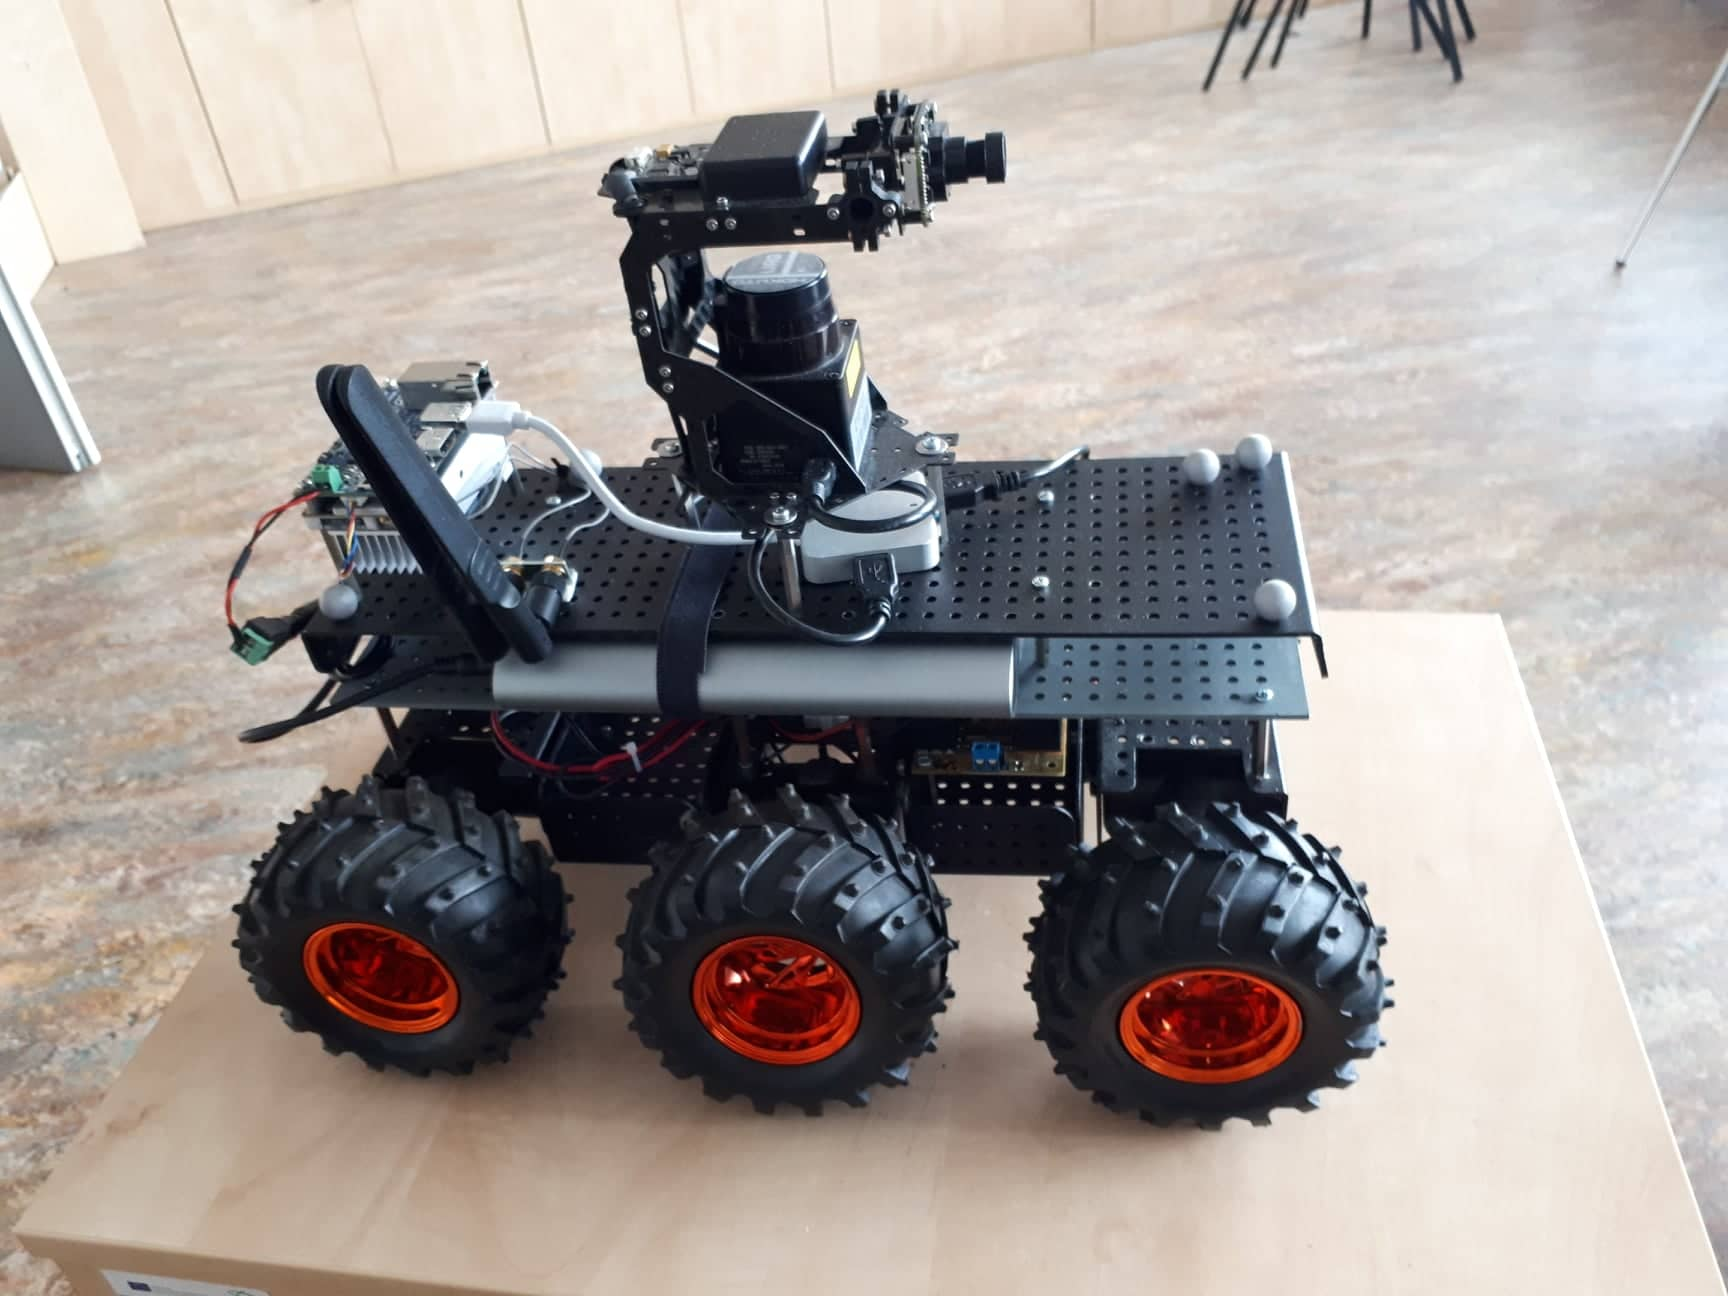
\includegraphics[width=0.7\columnwidth]{imgs/robot.jpg}
	\end{center}
	\caption{Dagu Wild Thumper 6WD s připevněnými senzory}
	\label{fig:robot}
\end{figure}


\subsection{Uložení trajektorie} \label{sekce:ulozeni_trajektorie}
Po nahrání datasetu a spuštěním všech metod SLAM na těchto datech, je získána množina výsledků, kterou je možno porovnat. Je více možností jak implementace porovnávat, kromě trajektorie je možné srovnání map. Pro možnost s mapou, byla by třeba tvorba výsledných map ve stejném měřítku a zisk přesné výměry prostředí, ve kterém byla data nahrána. Zvláště informace o přesné podobě prostředí by byla ve velkém množství porovnávání značný problém. Pro tyto účely se tak volí možnost s trajektoriemi, kdy zisk přesné trajektorie pohybu robota, $ground$ $truth$, je výrazně jednodušší.\\
\indent Tvorba trajektorie je u každého systému zcela rozdílná. Nejjednodušší extrakce trajektorie je v případě Hector SLAM. Tato metoda sama publikuje topik s názvem $slam\_out\_pose$, kde je zaznamenávána aktuální pozice. Tím, že Hector SLAM neumí přepisovat předchozí výsledky různými optimalizacemi, či uzavíráním smyčky a informace pouze přidává, může se $slam\_out\_pose$ při běhu implementace celou dobu poslouchat a data z topiku ukládat. Poslouchání topiku je prováděno příkazem \texttt{rostopic echo /topic}, což začne vypisovat data do terminálu. Přidáním za příkaz \texttt{> file.txt} se data uloží do daného soboru. Výsledný příkaz pro uložení trajektorie pomocí Hector SLAM tedy vypadá následovně:
\begin{center}
	\texttt{rostopic echo /slam\_out\_pose > trajectory\_hector.txt}
\end{center}
U metody gMapping je zisk trajektorie složitější. Tato implementace nikam trajektorii sama nezaznamenává. Jednou z možností, jak ji tedy získat, je využít uzel obsažený v systému Hector SLAM. Přidáním uzlu s názvem $hector\_trajectory\_server$ do spouštěného souboru $launch$ je tak získána možnost extrahovat trajektorii. Neboť je gMapping systém obsahující optimalizaci cesty a mapy a umí uzavírání smyčky, je třeba trajektorii uložit až po doběhnutí dat obsažených v souboru $bag$. Takto se zavolání topiku provádí příkazem \texttt{rosservice call /topic}, uložení do souboru se provede stejně jako v případě s Hector SLAM. Příkaz pro uložení trajektorie má podobu:
\begin{center}
	\texttt{rosservice call /trajectory > trajectory\_gmapping}
\end{center}
Nejsložitější postup zskávání trajektorie je v případě systému Cartographer. Dříve se dala tato informace získat pomocí dvou příkazů. Aktualizací Cartographeru před dvěma lety však zavedl Google pro ukládání dat nový formát $pbstream$, pro práci s nimž není příliš dobrá veřeně dostupná dokumentace. 
Cartographer při běhu publikuje uzel s názvem $/trajectory\_node\_list$, který nese v daném časovém okamžiku informaci o všech bodech trajektorie. Při dokončení výpočtů ze spuštěného $bag$ souboru je tedy k uložení dostupná finální trajektorie. Součástí této informace jsou však pouze souřadnice v prostoru a chybí tak informace o natočení, či časovém momentu, kdy robot v daném místě byl. Pro jednodušší porovnání implementací by to stačilo, ale pro správné porovnávání dle [11] by to bylo nedostatečné. Nakonec pro předevení souboru $pbstream$ do souboru $bag$ posloužil kód, který přidal do své implementace Cartographeru jeden výkumník Googlu [12]. V běžné implementaci Cartographeru se tento kód nevyskytuje. Využitím tohoto kódu již byla možnost trajektorii získat a to následujícím postupem. Nejprve je třeba nechat proběhnout všechny výpočty z nahraného souboru $bag$, pro lepší orientaci si bude označen jako $measured.bag$. Po doběhnutí výpočtů z $measured.bag$ je potřeba ukončit výpočty Cartographeru zavoláním
\begin{center}
	\texttt{rosservice call /finish\_trajectory 0},
\end{center}
kdy $0$ označuje číslo trajektorie. Tímto příkazem se zahrnou do optimalizace trasy a mapy i částice, na které při doběhnutí dat z $measured.bag$ ještě nedošlo. Následujícím příkazem
\begin{center}
	\texttt{rosservice call /write\_state state.pbstream},
\end{center} 
se uloží aktuální stav Cartographeru do souboru $pbstream$. Poté je třeba se dvěma parametry zavolat přidaný uzel s názvem $pbstream\_trajectories\_to\_bag$, který má dva vstupní parametry. První parametr je název souboru $pbstream$ a parametr druhý je název souboru $bag$, do kterého se data uloží. Tento nový $bag$ soubor bude pro orientaci nazýván jako $processed.bag$. Finálním krokem je z $processed.bag$ získání trajektorie, která je zde uložena v topiku $/tf$. To se provede již použitým příkazem \texttt{rostopic echo /topic}, za který se přidá argument \texttt{-b "bag\_file"}, čímž se řekne, že se nechce poslouchat aktuálně publikovaný topik, ale topik z určeného souboru $bag$. Za to se pro uložení do vybraného souboru ještě přidá \texttt{> file.txt}. Výsledný příkaz je tedy v podobě:
\begin{center}
	\texttt{rostopic echo /tf -b processed.bag > trajectory\_cartographer.txt}
\end{center}

\subsection{Příprava dat}
Data ze všech systémů jsou v stejném tvaru, počátek mají v bodě [0,0,0], informace o natočení má shodný počátek a i rozsah hodnot, který se pohybuje na intervalu $(0,1\rangle$. Stejně je tomu tak i v případě $ground$ $truth$, s jediným rozdílem, že počátek trajektorie není v bodě [0,0,0]. Úprava tak spočívala v posunutí všech bodů tak, aby byl počátek v tomto bodě.\\
Druhou a poslední úpravou, byla změna intervalu popisující natočení robota. Nově zvolený rozsah je $(-\pi,\pi\rangle$. Důvodem je problém se změnou natočení v okolí hraniční hodnoty. Při hodnotě natočení blízké jedné a otočením se na hodnotu blízké nule, vzniká velký rozdíl hodnot, který nepopisuje vzniklou situaci. S novým intervalem se může přeskočit od hodnoty blízké $\pi$ do hodnoty blízké $-\pi$, což při práci s absolutními hodnotami dává přesnou informaci o změně natočení. 

\newpage

\section{Vyhodnocení výsledků}
V této kapitole se nachází popis kritéria, dle kterého jsou porovnávány systémy SLAM. Následně jsou zde uvedeny výsledky z jednotlivých měření a jejich rozbor. 

\subsection{Srovnávací kritérium} \label{kapitola:comparison}
Pro srovnání algoritmů SLAM je dle [11] zvoleno porovnávací kritérium ve tvaru
\begin{equation}
	\varepsilon(\delta)=\varepsilon_{trans}(\delta)+\varepsilon_{rot}(\delta),
\end{equation}
kde $\varepsilon_{trans}(\delta)$ je chyba určení pozice robota a $\varepsilon_{rot}(\delta)$ je chyba natočení robota.\\
\indent Rovnice pro výpočet chyby pozice se dá dále rozepsat jako:
\begin{equation}
	\varepsilon_{trans}(\delta)=\frac{1}{N}\Sigma_{i,j}f_{trans}(\delta_{i,j}\ominus\delta^*_{i,j})^2,
\end{equation}
kde $N$ je celkový počet bodů trajektorie, $\delta_{i,j}$ je relativní pozice robota dle daného algoritmu SLAM v čase $i$ a $j$, přičemž $i$ a $j$ jsou bezprostředně se následující časové záznamy. Pozice v daných časových okamžicích z ground truth je označena jako $\delta^*_{i,j}$. Funkce $f_{trans}()$ je určena ve formě Euklidovské normy:
\begin{equation}
	f_{trans}(\delta_{i,j}\ominus\delta^*_{i,j})=||\delta_{i,j}\ominus\delta^*_{i,j}||
\end{equation}  
Rovnice pro určení chyby natočení robota je ve tvaru:
\begin{equation}
	\varepsilon_{rot}(\delta)=\frac{1}{N}\Sigma_{i,j}f_{rot}(\delta_{i,j}\ominus\delta^*_{i,j})^2,
\end{equation}
kde všechny proměnné mají stejný význam jako u chyby určení pozice a funkce $f_{rot}()$ má předpis:
\begin{equation}
	f_{rot}(\delta_{i,j}\ominus\delta^*_{i,j})=|min(2\pi-|\delta_{i,j}\ominus\delta^*_{i,j}|,|\delta_{i,j}\ominus\delta^*_{i,j}|)|
\end{equation}
Tento přístup, narozdíl od běžného porovnávání vzdálenosti bodů v prostoru, nehledí na přímý rozdíl pozice bodů v daném čase, ale na změnu relativních pozic v časovém úseku. 

\newpage
\subsection{Porovnání výsledků ze simulátoru Stage}
Pro porovnání výsledků, nahraných pomocí rozhraní Stage bylo vytvořeno několik obrázkových map. Přesnost algoritmů byla u všech map přibližně stejná. Názorné porovnání je tedy provedeno pouze na jedné, kde při průjezdu vznikly dvě smyčky. K porovnání jsou využity rovnice z předchozí sekce.\\
\begin{center}
	\begin{tabular}{c|ccp{3cm}}
		\bfseries \bfseries  & $\varepsilon_{trans}(\delta)$ $[m]$ & $\varepsilon_{rot}(\delta)$ $[rad]$ & $\varepsilon(\delta)$  \\ [2mm]
		\hline
		GMapping & $5.7225\times10^{-5}$ & $4.45249\times10^{-5}$ & $0.00010$  \\ 
		Hector & $4.12745\times10^{-5}$ & $0.00023$ & $0.00027$  \\ 
		Cartographer & $0.00086$ & $0.00062$ & $0.00149$  \\
	\end{tabular}
\end{center}

Z výsledků je zřejmé, že všechny algoritmy proběhly v pořádku a s vysokou přesností. Nejlepších výsledků v tomto případě dosáhl systém gMapping. Byla zde i prokázána důležitost zvoleného kritéria porovnávání. Například při srovnání trajektorií pomocí metody $Root$ $Mean$ $Square$ $Error$ (RMSE) dosáhl nejlepších výsledků algoritmus Hector SLAM. RMSE je porovnání trajektorií, kde se počítá pouze s rozdílem bodů v daném časovém okamžiku. 

\begin{figure}[!ht]
	\begin{center}
		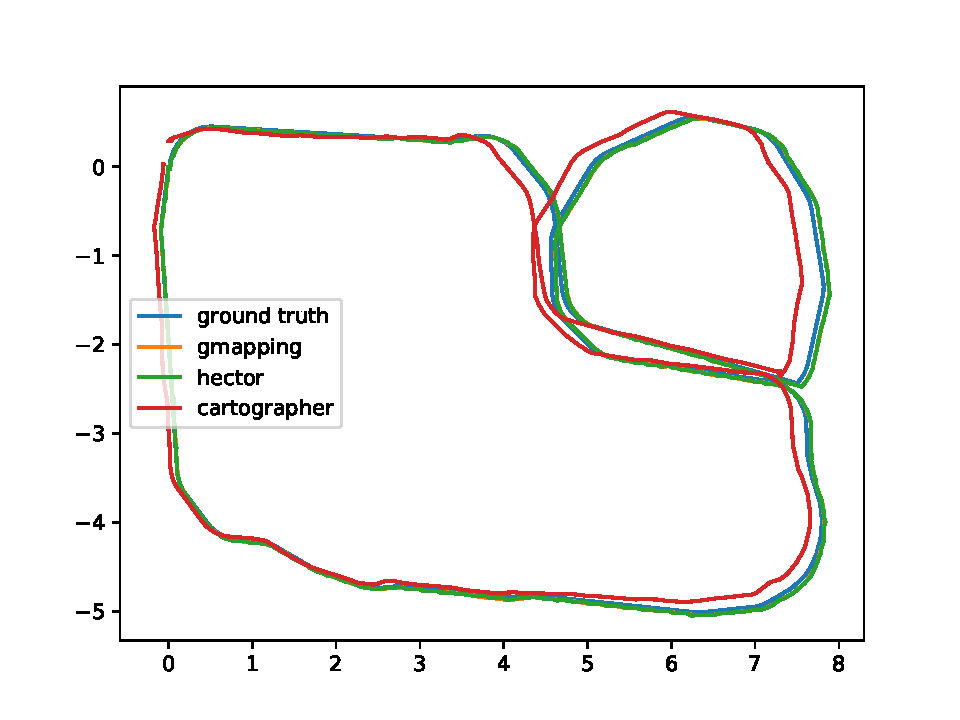
\includegraphics[width=0.7\columnwidth]{imgs/stage_trajectories.pdf}
	\end{center}
	\caption{Grafické srovnání vytvořených trajektorií}
	\label{fig:stage_trajectories}
\end{figure}

\begin{figure}[!ht]
	\begin{center}
		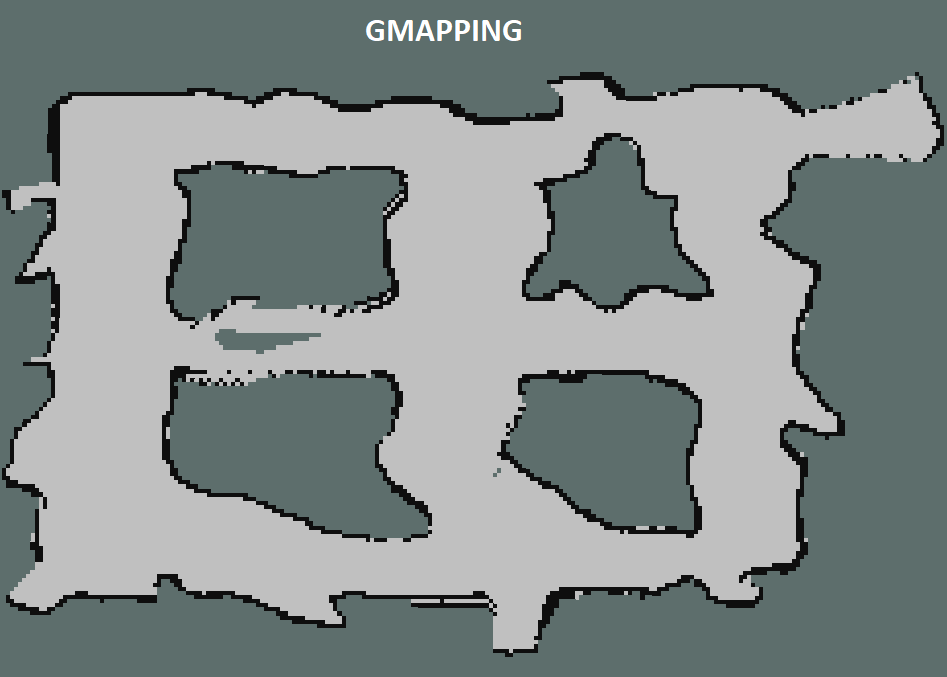
\includegraphics[width=0.5\columnwidth]{imgs/Maps/Bag/newmaze_with_ground_truth/gmapping_newmaze_with_ground_truth.png}
		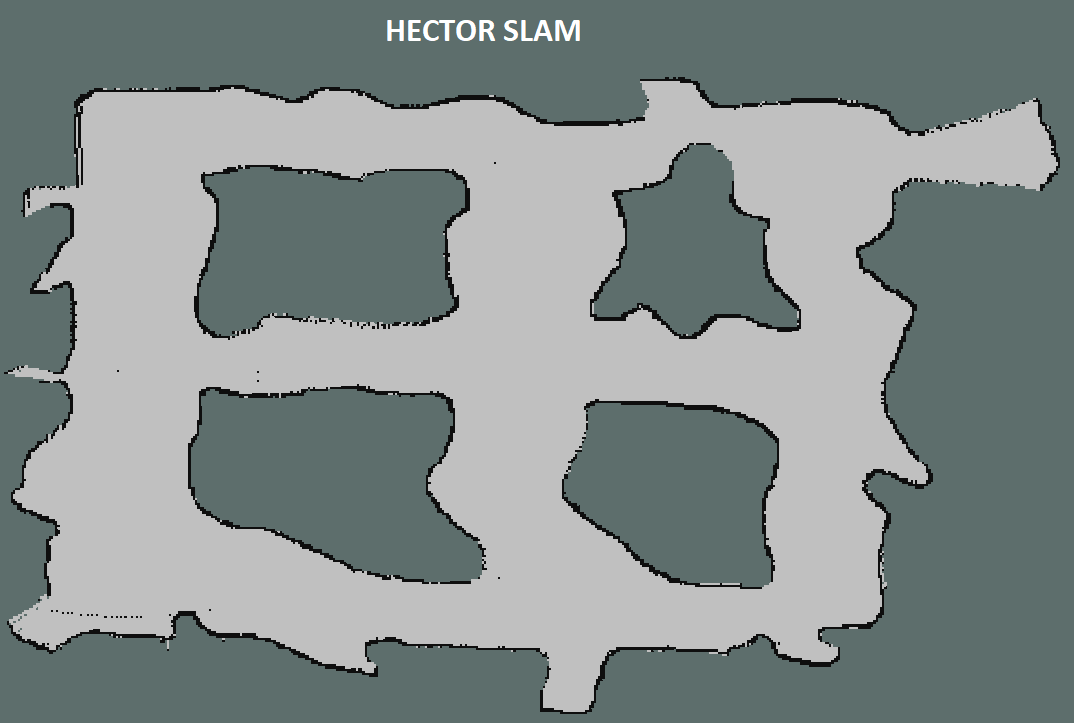
\includegraphics[width=0.5\columnwidth]{imgs/Maps/Bag/newmaze_with_ground_truth/hector_newmaze_with_ground_truth.png}
		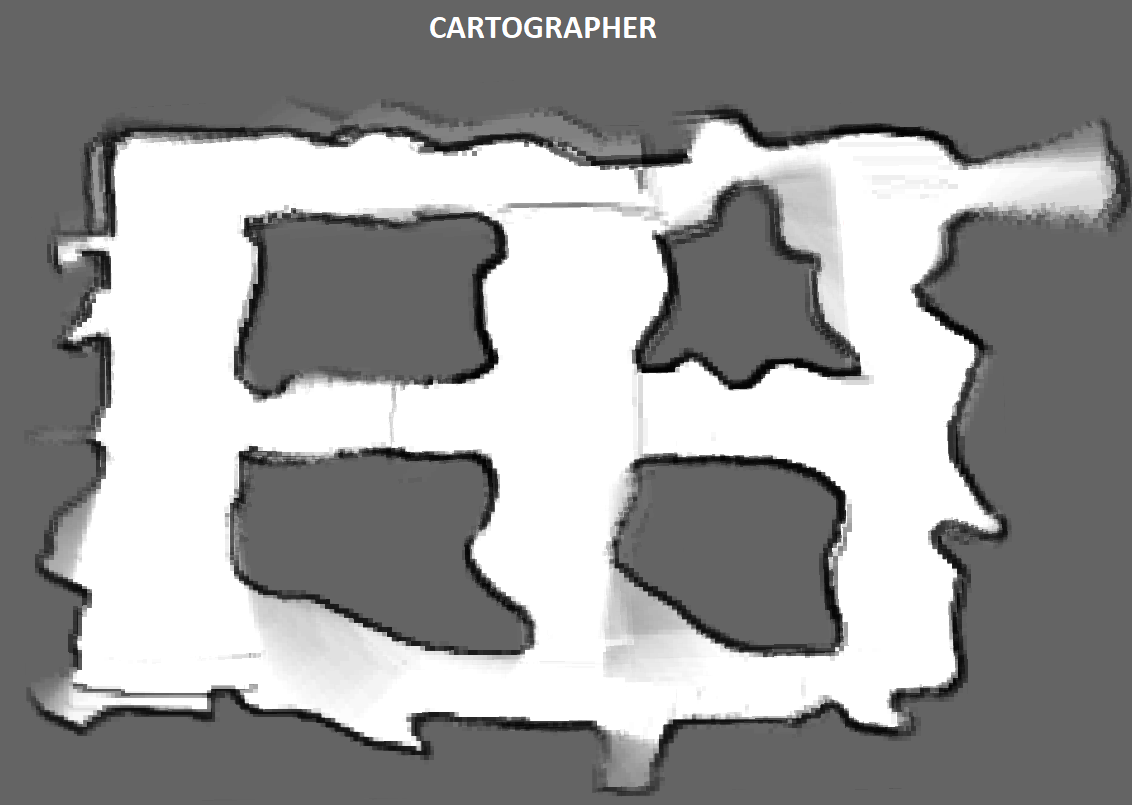
\includegraphics[width=0.5\columnwidth]{imgs/Maps/Bag/newmaze_with_ground_truth/cartographer_newmaze_with_ground_truth.png}
	\end{center}
	\caption{Vykreslené mapy jednotlivými systémy}
	\label{fig:mapy_stage}
\end{figure}

\newpage 

\subsection{Porovnání výsledků ze staženého datasetu}
Pro porovnání systémů byla potřeba najít dataset, který v sobě obsahuje všechny potřebné informace pro jejich vykonání. Další podmínkou, která musela být splněna, aby testování mělo srovnatelné výsledky, je nutnost znalosti $ground$ $truth$ pro daná data. Potřebné informace obsahují datasety nahrané v MIT Stata Center, kde k mnohým z nich je možno ještě stáhnout zmíněné $ground$ $truth$. Pro porovnání tak byl zvolen jeden z těchto datasetů.\\
\indent $Ground$ $truth$ má rovnou informaci o natočení v rozsahu $(-\pi,\pi\rangle$, nebyla v tomto  ohledu tedy potřeba žádná změna. Data však byla natočená přibližně o 30$^o$ a posunuta mimo počátek [0,0,0]. Stažená data byla tedy přepočítána tak, aby bylo natočení a počátek stejný. Porovnávání pak bylo provedeno dle rovnic v kapitole \ref{kapitola:comparison}.\\
\begin{center}
	\begin{tabular}{c|ccp{3cm}}
		\bfseries \bfseries  & $\varepsilon_{trans}(\delta)$ $[m]$ & $\varepsilon_{rot}(\delta)$ $[rad]$ & $\varepsilon(\delta)$  \\ [2mm]
		\hline
		GMapping & $0.02002$ & $0.00698$ & $0.02701$  \\ 
		Hector & $0.00860$ & $0.00144$ & $0.01005$  \\ 
		Cartographer & $0.00049$ & $0.00148$ & $0.00197$  \\
	\end{tabular}
\end{center}

\begin{figure}[!ht]
	\begin{center}
		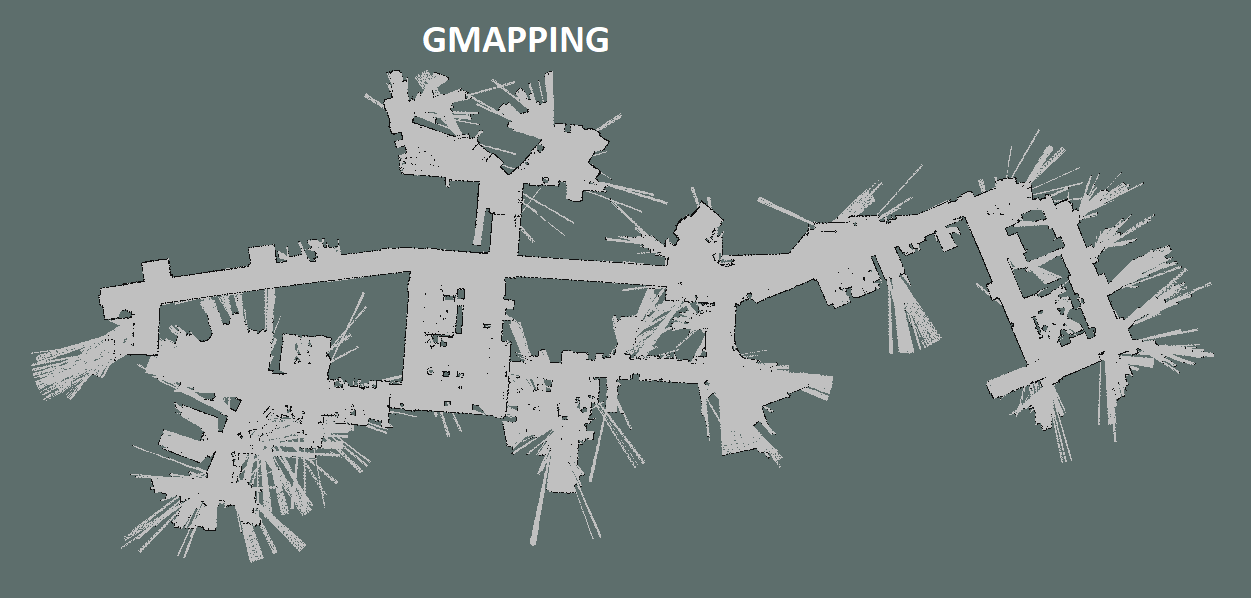
\includegraphics[width=0.6\columnwidth]{imgs/Maps/Bag/mit_stata_short/gmapping_mit_stata_short.png}
		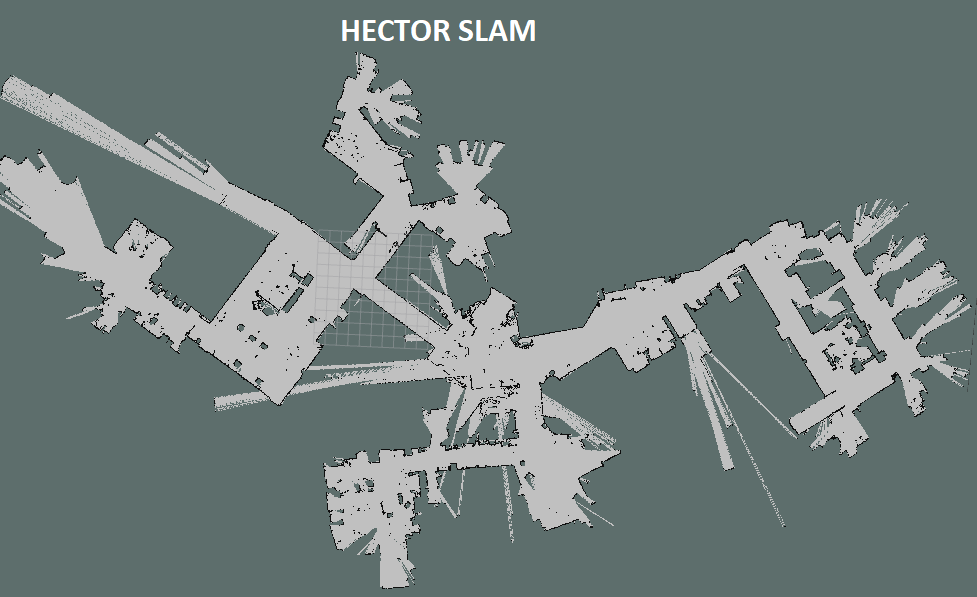
\includegraphics[width=0.6\columnwidth]{imgs/Maps/Bag/mit_stata/hector_mit_stata.png}
		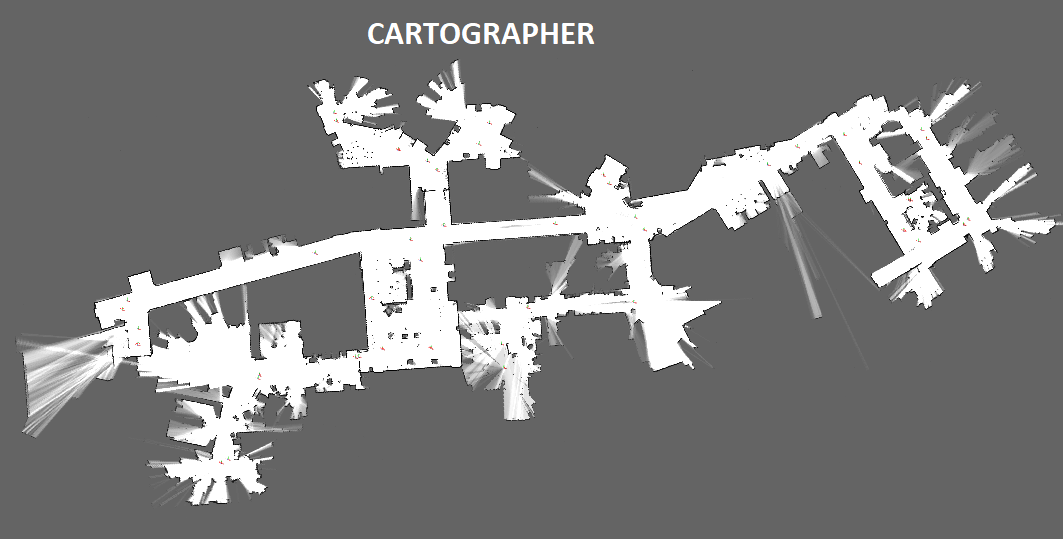
\includegraphics[width=0.6\columnwidth]{imgs/Maps/Bag/mit_stata_short/cartographer_mit_stata_short.png}
	\end{center}
	\caption{Vykreslené mapy jednotlivými systémy pro zkrácený dataset}
	\label{fig:mapy_mit_short}
\end{figure}

Z výsledků je patrné, že v tomto případě si nejlépe vedl Cartographer. Za ním je dle tabulky Hector SLAM a poslední je gMapping. Při pohledu na mapu je však vidět, že trajektorie Hector SLAMu je neúplná a na konci silně vychýlená. Je to z důvodu, že při průjezdu předcházejícím výběžkem, došlo vždy k dislokaci robota, následně i v dalších částech měl problémy v orientaci i přes změny v řadě nastavení. Trajektorie Hector SLAMu by tak byla pro porovnání naprosto nevyhovující a je proto ukončena v bodě, do kterého se systém jevil správně. Grafické znázornění na obrázcích \ref{fig:mit_short}, \ref{fig:mapy_mit_short}\\

\begin{figure}[!ht]
	\begin{center}
		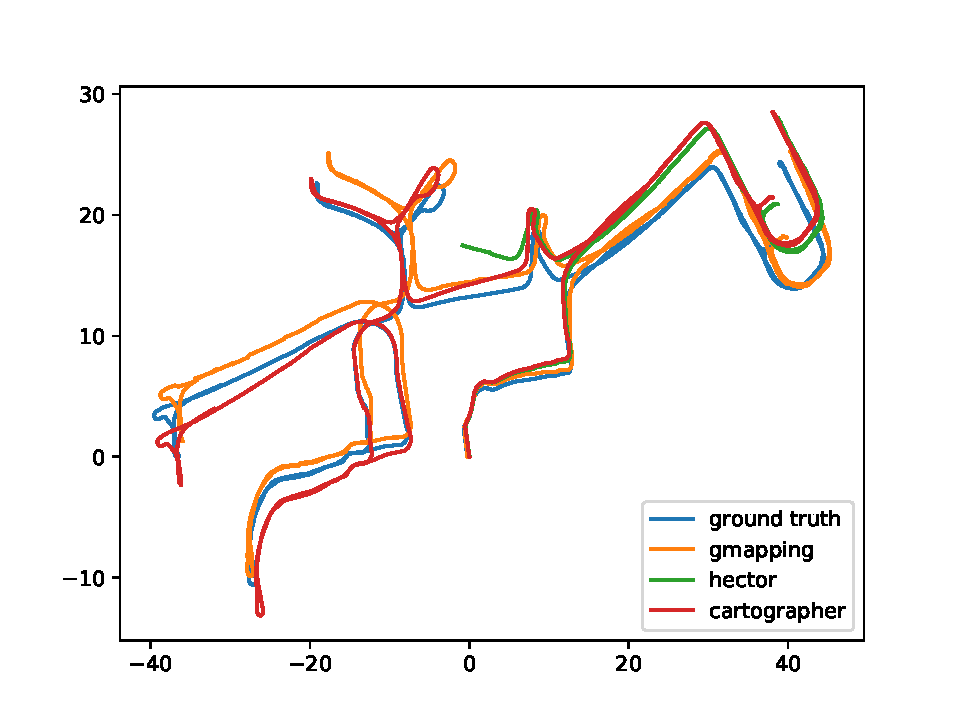
\includegraphics[width=0.7\columnwidth]{imgs/mit_short.pdf}
	\end{center}
	\caption{Grafické srovnání vytvořených trajektorií pro zkrácený dataset}
	\label{fig:mit_short}
\end{figure}

\indent Výše zmíněné výsledky a mapy, jsou však získány z datasetu, kterému byla zmenšena obsažená data. Respektive jsou od určitého času ustřižena. Důvod byl, že i přes nastavení Cartographeru určené pro tyto data, nedokázal si tento systém částečně poradit s jednou chodbou a došlo tak k posunu velké části trajektorie a mapy (dané místo znázorněno na mapách náležících obrázku \ref{fig:mapy_mit_full}). Výsledky z celého datasetu jsou následující.\\
\begin{center}
	\begin{tabular}{c|ccp{3cm}}
		\bfseries \bfseries  & $\varepsilon_{trans}(\delta)$ $[m]$ & $\varepsilon_{rot}(\delta)$ $[rad]$ & $\varepsilon(\delta)$ \\ [2mm]
		\hline
		GMapping & $0.02601$ & $0.00831$ & $0.03432$ \\ 
		Cartographer & $0.00292$ & $0.00158$ & $0.00451$ \\
	\end{tabular}
\end{center}

Je vidět, že výsledky se u obou porovnávaných systémů mírně zhoršily, chyba v pozici u Cartographeru poté výrazněji, což je zaviněno zmíněným posunem. I tak má však Cartographer opět lepší výsledek, neboť srovnávací kritérium nepočítá rozdíl jednotlivých bodů od sebe, ale poměřuje přírůstek mezi dvěma časovými okamžiky. Přechody v trajektorii jsou u Cartographeru tedy přesnější, než ty u gMappingu. 
\newpage
\begin{figure}[!ht]
	\begin{center}
		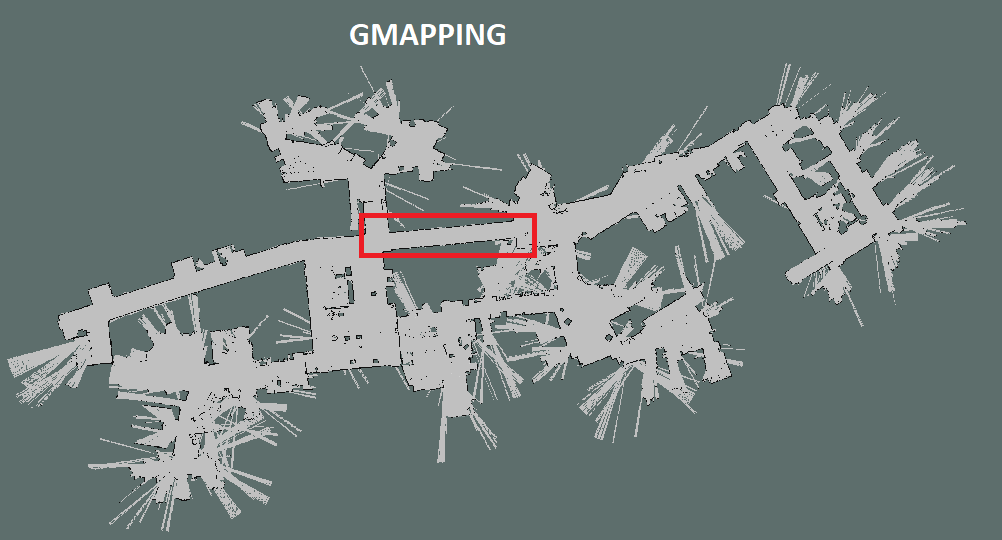
\includegraphics[width=0.6\columnwidth]{imgs/Maps/Bag/mit_stata/gmapping_mit_stata.png}
		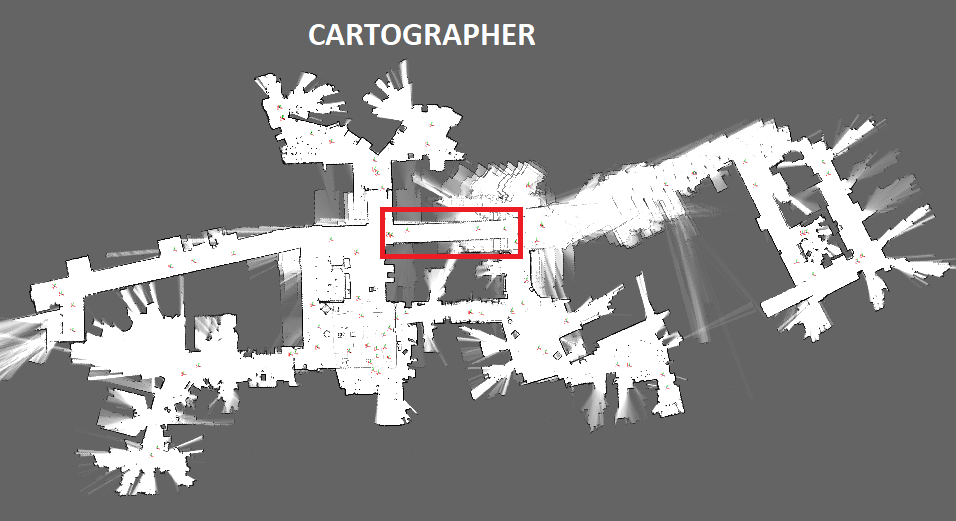
\includegraphics[width=0.6\columnwidth]{imgs/Maps/Bag/mit_stata/cartographer_mit_stata.png}
	\end{center}
	\caption{Vykreslené mapy jednotlivými systémy pro celý dataset}
	\label{fig:mapy_mit_full}
\end{figure}

\begin{figure}[!ht]
	\begin{center}
		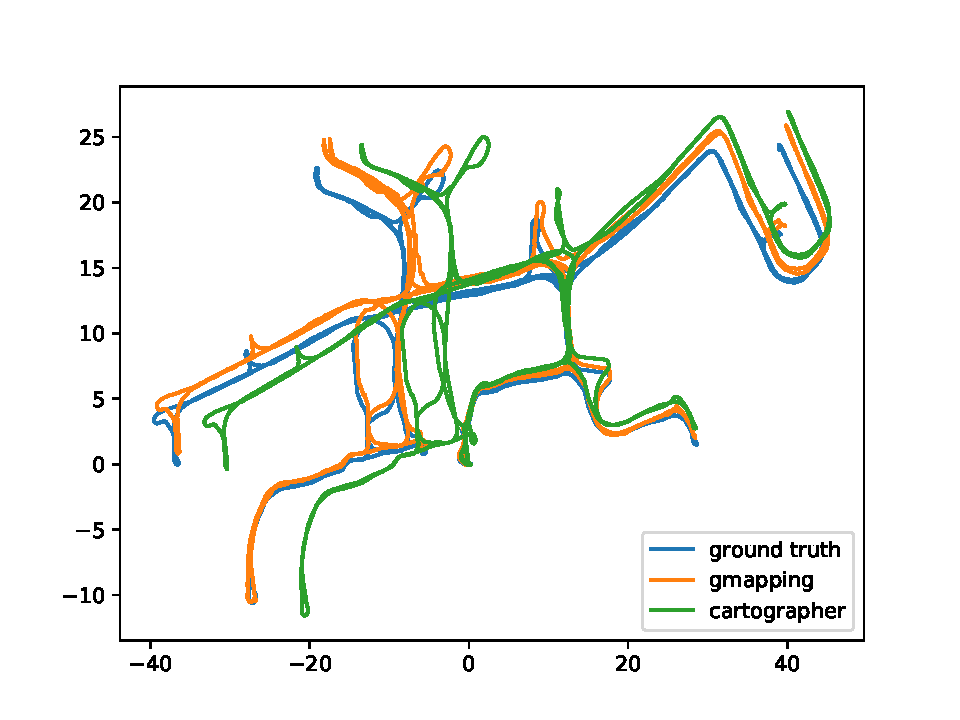
\includegraphics[width=0.7\columnwidth]{imgs/mit_full.pdf}
	\end{center}
	\caption{Grafické srovnání vytvořených trajektorií pro celý dataset}
	\label{fig:mit_full}
\end{figure}

\subsection{Porovnání dat nahraných robotem} \label{sekce:data_robot}
Data pro toto porovnání jsou nahrána na Fakultě aplikovaných věd ZČU v budově NTIS. Jak je již výše zmíněno, odometrie zaznamenána robotem je v tomto případě nepoužitelná. Přesto, že vše v něm nahrané je nastaveno dle specifikace výrobce, informace je velmi nepřesná. Robot sám při jízdě dopředu lehce zatáčí doprava. Informace o dopředném pohybu je ale jinak ukládána správně, při zatáčení však robot zaznamenává informaci o mnohem větším zatočení, než k jakému došlo. Ztráta odometrie má na každý ze systémů rozídlný dopad.\\
\indent Hector SLAM, který odometrickou informaci vůbec nepoužívá, není tedy tímto omezením nijak ovlivněn a jeho průběh je standardní. Cartographer již odometrii využívá, lze ale vypnout sledování odometrie a používat odometrii systémem dopočítávanou. Použitím tohoto nastavení se Cartographer stává náchylný na podlouhlé prostory bez větších rodílů, typickým příkladem jsou chodby. GMapping bezpodmíněčně odometrickou informaci vyžaduje. Informace silně zkreslená tak průběh programu velmi komplikuje.\\
\indent Při pohledu na vytvořené mapy (obrázek \ref{fig:mapy_robot}) je znát nedostatek s odometrií pouze u Cartographeru, kdy jedno projetí celého prostoru bylo nedostatečné a mapa není na pohled příliš kvalitní. Pro srovnání jsem však nahrál ještě nový dataset, kdy jsem projel daný prostor dvakrát a výsledek je znatelně lepší.(obrázek \ref{fig:mapa_robot_cartographer_dvakrat})\\
\indent Pohled na trajektorie je však již více vypovídající o nedostatcích spojených s nekvalitní odometrickou informací. Pro Hector SLAM se opět nic neměnilo a trajektorie je v pořádku. U Cartographeru je vidět, že kvůli občasným problémům s rozeznáním posunu po chodbách, je trajektorie značně kratší. Největší problém v oblasti trajektorie je znatelný u systému gMapping, kdy informace o přetáčení vytváří na trajektorii po celou dobu velké výchylky a zuby. Algoritmus si s tím však dokáže i tak poradit a výsledná mapa tím ovlivněna není.\\
\indent Bez znalosti $ground$ $truth$ je třeba porovnat algoritmy na základě získaných map. Měřením poměru vzdáleností mezi jednotivými body v prostoru a porovnáním s těmito body ve vytvořených mapách, vychází pro tento případ jako nejlepší algoritmus Hector SLAM, v těsném závěsu poté gMapping. Pro srovnání je přiložen i graf s trajektoriemi \ref{fig:robot_trajectory}. 



\begin{figure}[!ht]
	\begin{center}
		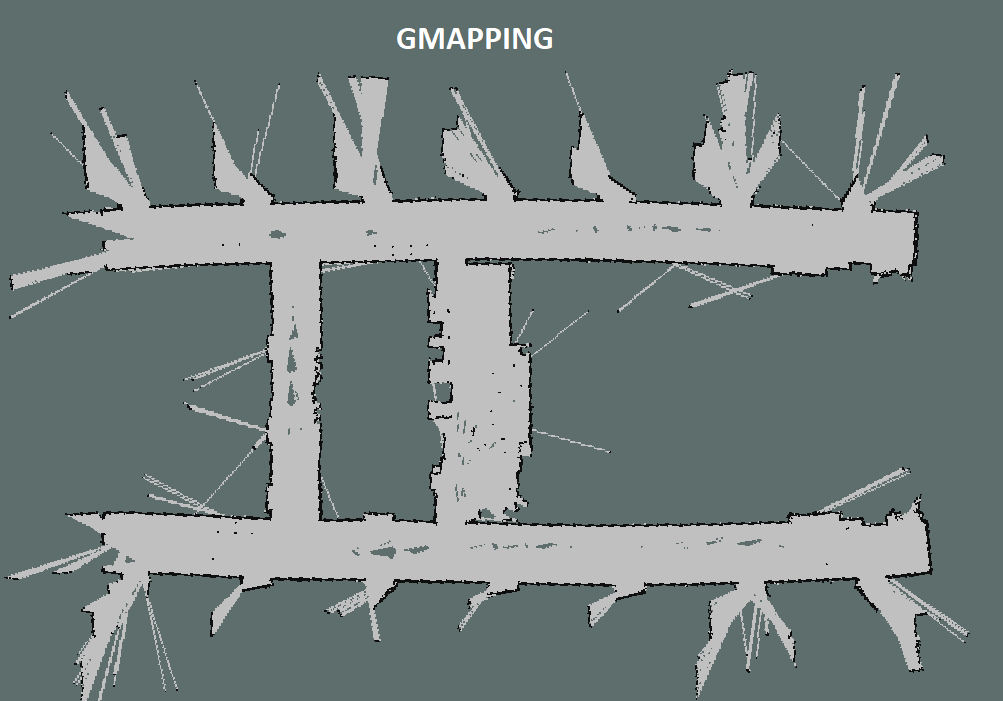
\includegraphics[width=0.6\columnwidth]{imgs/Maps/Robot/5patromoreslower/gmapping_5patromoreslower.png}
		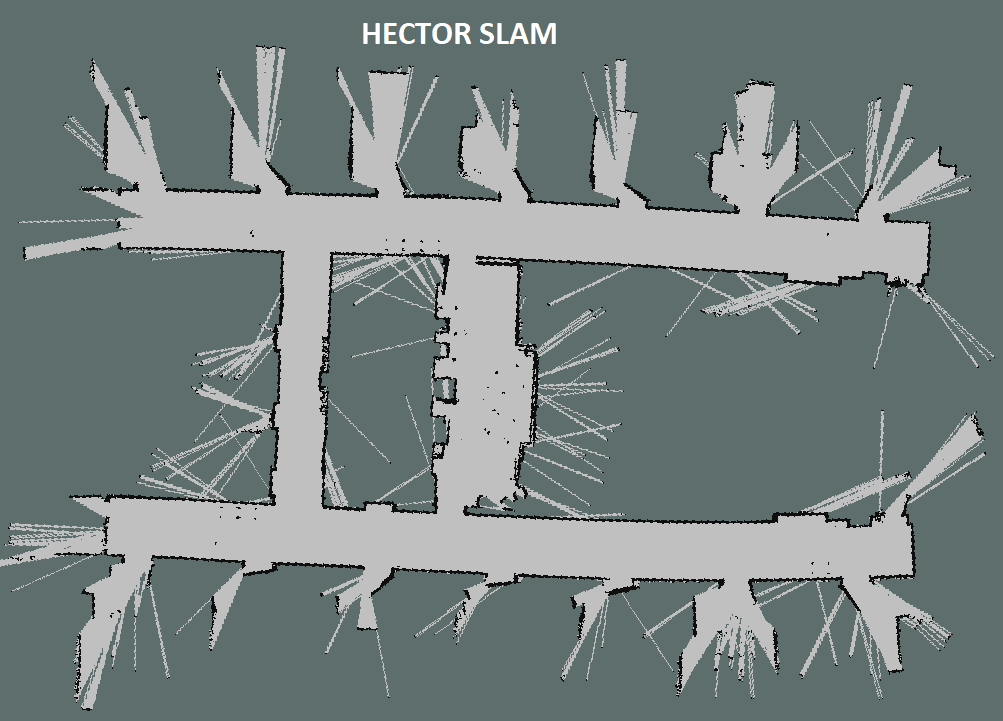
\includegraphics[width=0.6\columnwidth]{imgs/Maps/Robot/5patromoreslower/hector_5patromoreslower.png}
		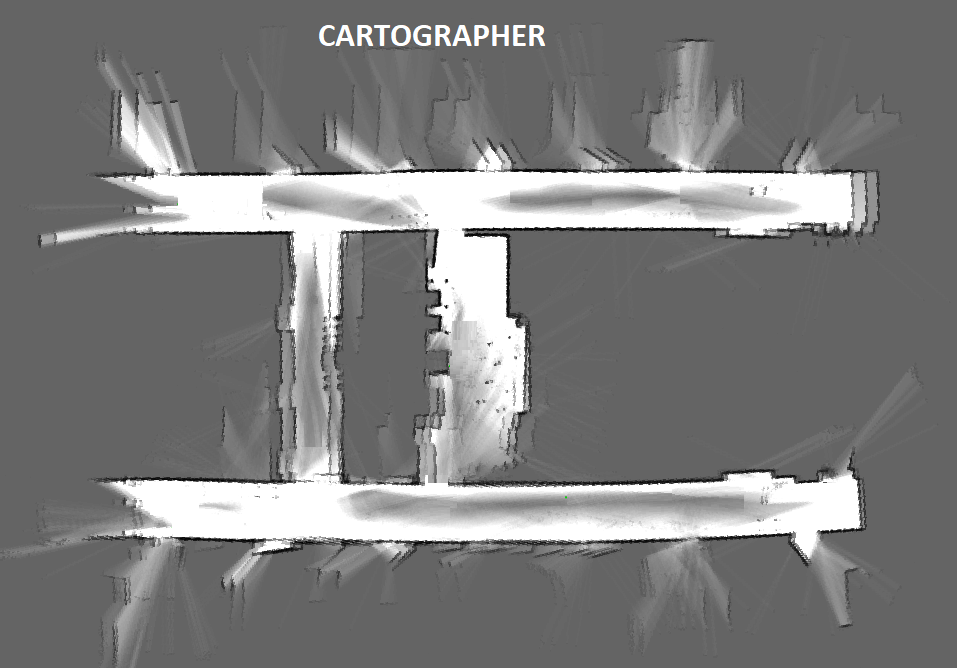
\includegraphics[width=0.6\columnwidth]{imgs/Maps/Robot/5patromoreslower/cartographer_5patromoreslower.png}
	\end{center}
	\caption{Vykreslené mapy jednotlivými systémy pro nahraná data robotem}
	\label{fig:mapy_robot}
\end{figure}

\begin{figure}[!ht]
	\begin{center}
		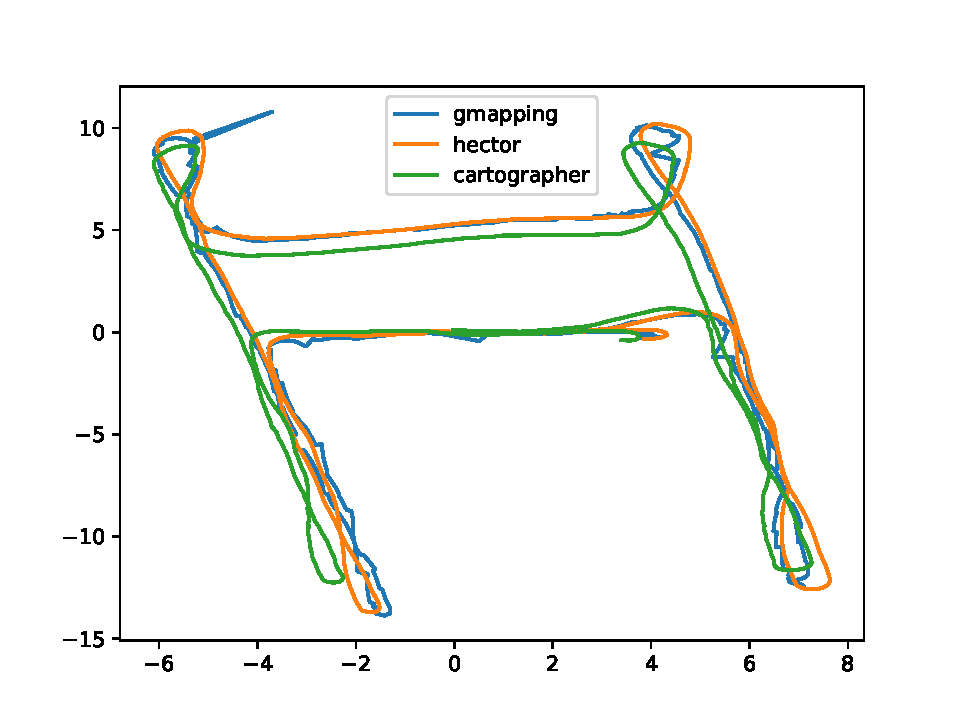
\includegraphics[width=0.7\columnwidth]{imgs/robot_trajectory.pdf}
	\end{center}
	\caption{Trajektorie jednotlivých systémů vytvořené na datech nahraných robotem}
	\label{fig:robot_trajectory}
\end{figure}

\begin{figure}[!ht]
	\begin{center}
		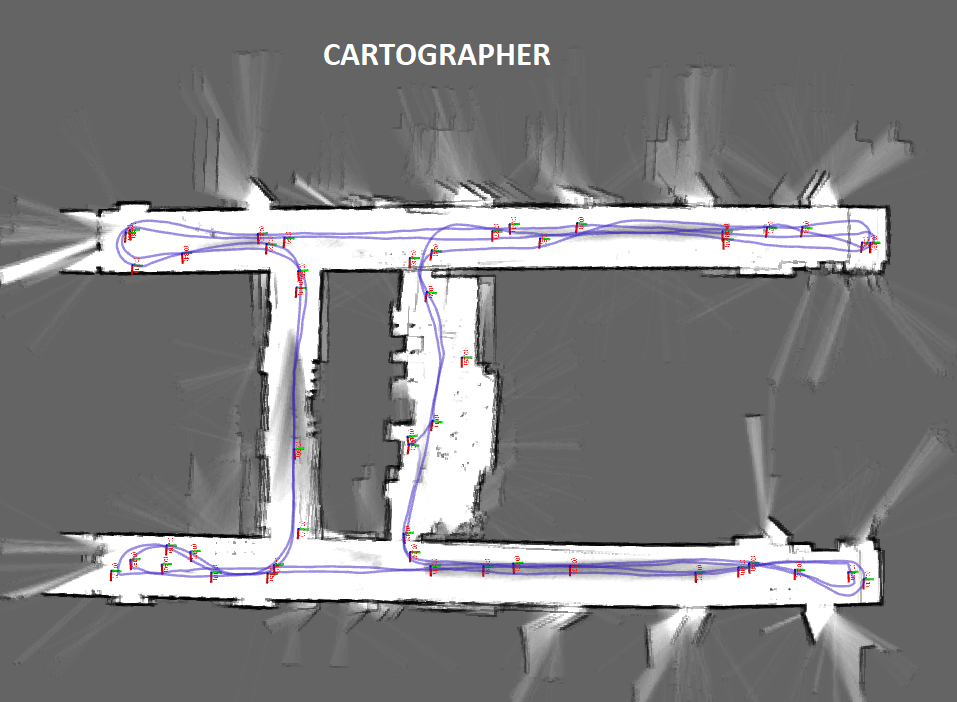
\includegraphics[width=0.6\columnwidth]{imgs/Maps/Robot/5patrodvakrat_cart_traj.png}
	\end{center}
	\caption{Mapa vytvořená systémem Cartographer při dvojném projetí protoru}
	\label{fig:mapa_robot_cartographer_dvakrat}
\end{figure}

\newpage

\chapter{Průzkum vybraného systému}
Pro důkladnější prozkoumání vybraného systému byl zvolen gMapping, neboť je nejstarší, má aktivní komunitu a stále se využívá. Tím je zajištěno rychlé ustabilizování systému po případných aktualizacích. Pro bližší seznámení a případné návrhy změn vychází tedy nejlépe.

\section{Změny v konfiguraci systému}
V předchozích měřeních bylo vždy použito defaultní nastavení systému. Toto nastavení nebylo třeba měnit, neboť gMapping vždy provedl výpočty dle očekávání a nikdy se nestalo, že by jako jediný selhal. Pro zkoumání vlivu nastavení na systém, byly postupně měněny různé parametry. Jako testovací data byl zvolen zkrácený dataset z MIT Stata Center.\\
\indent Kritériem pro testování vlivu nastavení na algoritmus byla pro tento případ zvolena odlišná rovnice, která porovnává přímo polohu jednotlivých bodů trajektorie s $ground$ $truth$ ($Root$ $Mean$ $Square$ $Error$). Důvodem je absence extrahovatelné trajektorie přímo ze systému gMapping. Při vývoji tak nebyl kladen důraz na srovnání dle [11], ale hlavně na to, aby částice tvořící mapu měli správné umístění. Rovnice použitá pro srovnání je ve tvaru:
\begin{equation}
	e(t,g)=\sqrt{\frac{1}{N}\Sigma_i(||t_i-g_i||)^2},
\end{equation}
kde $t$ je vypočtená trajektorie, $g$ je $ground$ $truth$, $N$ je počet vzorků trajektorie a $i$ udává časový okamžik.\\
\indent V násedující tabulce jsou defaultní hodnoty parametrů, které byly upraveny pro účely porovnání. Ostatní parametry byly ponechány na defaultních hodnotách. 
\begin{center}
	\begin{tabular}{c|c|p{9.5cm}}
		\bfseries Parametr  & \bfseries Hodnota & \bfseries Význam \\ [2mm]
		\hline
		$linearUpdate$ & $1.0$ & ujetá vzdálenost pro nové měření [m]  (1)\\
		$angularUpdate$ & $0.5$ & zaznamenané otočení pro nové měření [rad]\\
		\hline
		$particles$ & $30$ & počet částic tvořený v každém kroce  (2)\\
		\hline
		$llsamplerange$ & $0.01$ & rozsah translačního vzorkování pravděpodobnosti (3)\\
		$llsamplestep$ & $0.01$ & krok v translačním vzorkování pravděpodobnosti\\
		$lasamplerange$ & $0.005$ & rozsah úhlového vzorkování pravděpodobnosti\\
		$lasamplestep$ & $0.005$ & krok v úhlovém vzorkování pravděpodobnosti\\
	\end{tabular}
\end{center}
Číselná hodnota vpravo u prvního parametru v dané sekci znázorňuje označení dané skupiny. Provedená měření se prováděla vždy se změnou parametrů pro celou skupinu.
Výsledky pro první skupinu:
\begin{center}
	\begin{tabular}{cc|p{1.5cm}}
		\bfseries $linearUpdate$  & \bfseries $angularUpdate$ & $e(t,g)$ \\ [2mm]
		\hline
		0.1 & 0.05 & 1.318 \\
		0.5 & 0.25 & 1.519 \\ 
		1 & 0.5 & 1.436 \\ 
		2 & 1.0 & 1.132 \\
		4 & 1.25 & 1.460\\
	\end{tabular}
\end{center}
Z této tabulky je vidět, že ve většině případů nemá dané nastavení velký vliv na průběh programu. S nastavením na $linearUpdate=2$ a $angularUpdate=1$ je však dosaženo znatelného zlepšení. Snížením vzorkování dochází ke snížení výkonových nároků, ale stále je udržena dostatečná frekvence pozorování pro správné sestavení mapy. Pro tento případ tedy dané nastavení zlepšuje průběh programu.\\

\begin{figure}[!ht]
	\begin{center}
		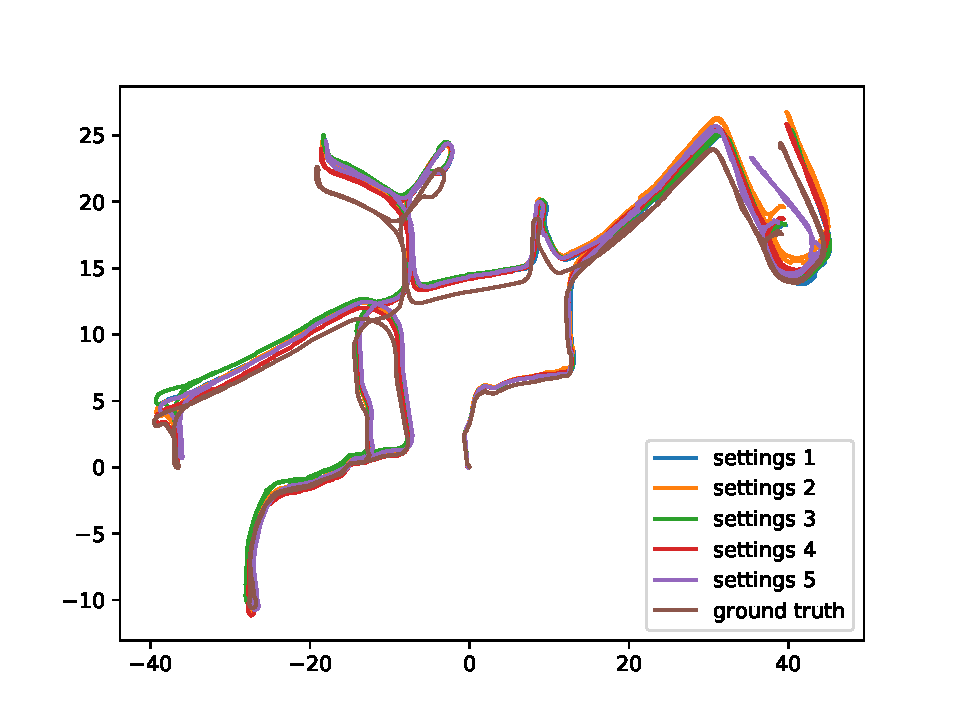
\includegraphics[width=0.67\columnwidth]{imgs/gmapping1.pdf}
	\end{center}
	\caption{Získané trajektorie pro první skupinu nastavení}
	\label{fig:gmapping1}
\end{figure}

\indent Pro druhou sadu nastavení se měnil pouze parametr $particles$:
\begin{center}
	\begin{tabular}{c|p{1.5cm}}
		\bfseries $particles$  & $e(t,g)$ \\ [2mm]
		\hline
		15 & 1.567\\
		30 & 1.436 \\ 
		45 & 1.433 \\
	\end{tabular}
\end{center}
Ze zdejších výsledků je znatelné, že se průběh programu s počtem vytvářených částic zlepšoval. Jedná se o logický krok, kdy by mělo docházet k úměře počtu částic a přesnosti trajektorie. Čím více částic je produkováno, tím je větší šance, že je vytvořena částice bližší reálným souřadnicím. Naproti tomu se s přibývajícími částicemi zvyšují výkonnové nároky programu, proto se nemůže nastavovat tento parametr na příliš vysoké hodnoty.\\
\begin{figure}[!ht]
	\begin{center}
		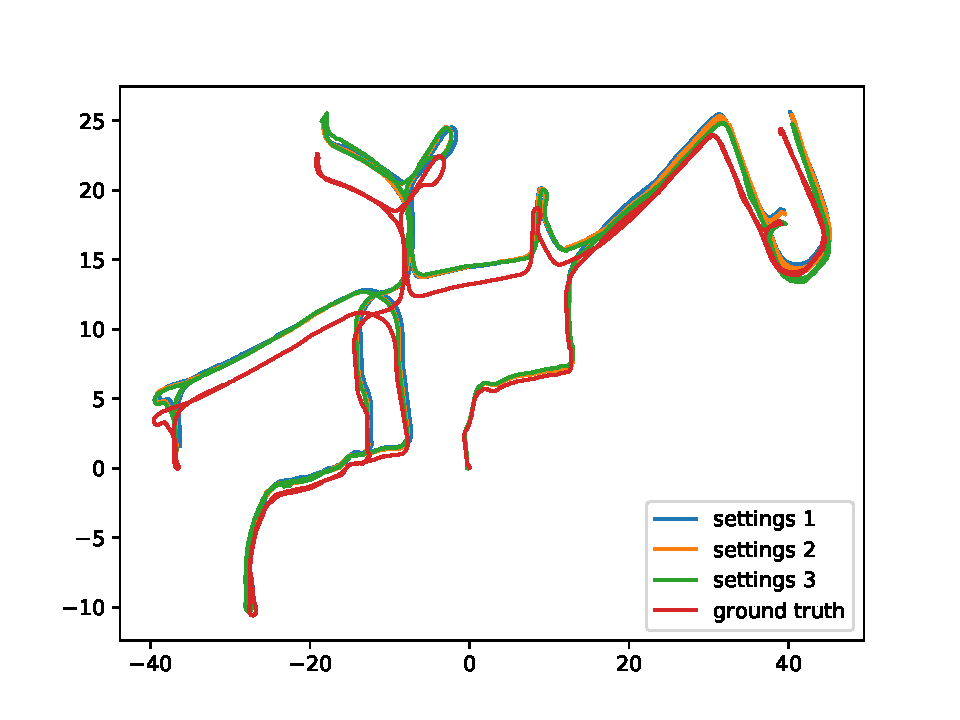
\includegraphics[width=0.67\columnwidth]{imgs/gmapping2.pdf}
	\end{center}
	\caption{Získané trajektorie pro druhou skupinu nastavení}
	\label{fig:gmapping2}
\end{figure}

\indent V poslední testované skupině se měnily parametry pro vzorkování pravděpodobnosti:
\begin{center}
	\begin{tabular}{cccc|p{1.5cm}}
		\bfseries $llsamplerange$  & \bfseries $llsamplestep$ & \bfseries $lasamplerange$ & \bfseries $lasamplestep$ & $e(t,g)$ \\ [2mm]
		\hline
		0.001 & 0.001 & 0.0005 & 0.0005 & 1.742 \\
		0.005 & 0.005 & 0.001 & 0.001 & 1.568 \\ 
		0.01 & 0.01 & 0.005 & 0.005 & 1.436 \\ 
		0.1 & 0.1 & 0.05 & 0.05 & 1.256 \\
		0.5 & 0.5 & 0.2 & 0.2 & 1.250\\
	\end{tabular}
\end{center}
Z posledních výsledků je patrné, že přes častější vzorkování není v tomto případě dosaženo lepších výsledků. Důvodem jsou opět zmiňované výkonnostní nároky, které byly s častějším vzorkováním příliš vysoké.\\
\indent Z těchto informací lze dojít k závěru, že systém je defaultně dobře nastavený na výkonější zařízení. Jednotlivá nastavení lze upravit tak, aby algoritmus poskytnul lepší výsledek, při kombinaci více parametrů dohromady však již vzniká riziko zvýšení výkonnových nároků natolik, že má změna nastavení na program opačný vliv.

\begin{figure}[!ht]
	\begin{center}
		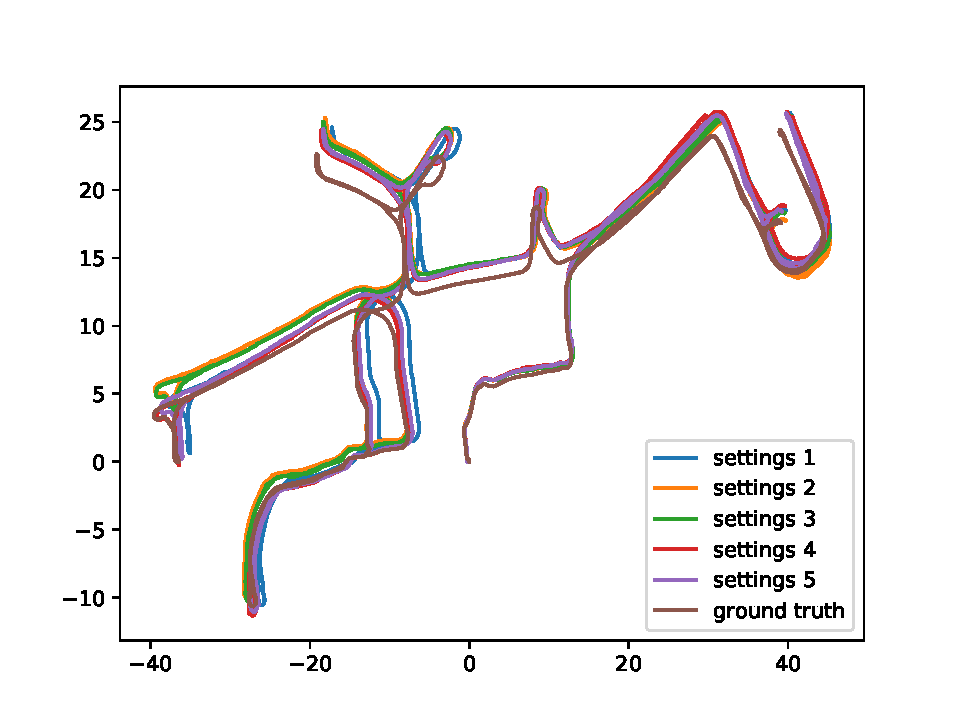
\includegraphics[width=0.67\columnwidth]{imgs/gmapping3.pdf}
	\end{center}
	\caption{Získané trajektorie pro třetí skupinu nastavení}
	\label{fig:gmapping3}
\end{figure}

\newpage
\section{Návrh změn v systému} \label{kapitola:navrh zmen}
Jako první věc, kterou je dobré uvést, je výše zmíněná neprodukce extrahovatelné trajektorie. Jako řešení se zde nabízí přidání topiku, který bude mít podobnou strukturu jako $/trajectory\_node\_list$ v Cartographeru. Tento topik, jak je popsáno v kapitole \ref{sekce:ulozeni_trajektorie}, nemá však pro potřebné porovnávání dostatek informací. Pro případ gMappingu by tak mohl být publikován topik, který by posílal v daném čase informaci o aktuální trajektorii. Obsah topiku by tak obsahoval vždy hlavu, ve které by byl uvedený aktuální čas. K tomu by byly připojeny pod sebou dle času seřazené částice tvořící aktuální trajaketorii. K těmto částicím by byla přidružena vždy informace o simulačním čase, kdy byla částice vytvořena, její souřadnice v prostoru a informace o natočení. Při poslouchání topiku v průběhu programu by tak bylo možné získat srovnání, jak se trajektorie v průběhu času optimalizovala. Při zavolání po doběhnutí datasetu by pak byla poskytnuta rovnou hotová trajektorie.\\
\indent Další prospěšnou změnou by pro systém byla určitě možnost upravovat parametry za běhu programu. Pro výše provedené testy nebyla taková úprava potřeba, neboť se jak reálný, tak simulační robot pohybovali po celou dobu ve stejném prostředí. Při uvážení, že by se však robot přemisťoval mezi uzavřenými a otevřenými prostory, tato mořnost by byla jistě užitečná. Při běžněm průběhu, kdy uživatel robotem sám jezdí, může program vypnout a spustit gMapping s jiným nastavením, což není příliš hezké řešení. Pro autonomního robota by to však mohl být větší problém. V případě, že vyjede do jiného typu prostředí mohl by si sám přenastavit parametry tak, aby odpovídali již někde uloženému nastavení pro dané prostředí.\\
\indent Zlepšení systému by bylo jistě dosaženo i integrací jednotky IMU, která by zajišťovala zlepšení odhadu pozice. V jednotce IMU jsou obsaženy gyroskopy, akcelerometry a magnetometry, které zjišťují stoupání, vybočení a rolování. Zaznamenáváním zmíněných hodnot je tedy získán lepší přehled o pohybu robota, než pouze z odometrie kol a tím tedy zlepšení odhadu pozice.\\
\indent Další potenciální změnou, která se již nevztahuje přímo k procesům v gMappingu, by byla integrace kamerového vidění, například monokulární kamery. Robot by snímal prostředí jak LIDARem, tak kamerou. V případě kamerových dat by se snažil rozeznat předměty v prostoru a následně předat informaci o tom, jaký typ předmětu to je. Například při detekci židle by byla vyslána informace, že se daný předmět nemá zanášet do mapy, případně z mapy vymazat. Do místa, kde je židle postavena, by se ještě přidala značka substituující židli. Při opětovném projetí by pak robot věděl, že v daném místě by se mohla židle nacházet a v případě, že tam stále nějaký předmět je, rovnou se snažit ho označit jako židli. Při velké množině objektů v paměti by se tak ušetřilo mnoho výpočetního výkonu. "Pohyblivé" předměty jsou v mapě navíc a při jejich přemístění může mít robot problém poznat stejné místo. Pokud by tedy v mapě zaneseny nebyly a robot měl opět jak LIDAR, tak kameru, sám by opět vyhodnotil, že předměty jsou v prostoru navíc, a počítal by tak s mapou předměty neobsahující. Pokud by mu tak byla poskytnuta mapa nějakého takto "vyčištěného" prostředí, byl by v něm schopen určit svoji pozici bez ohledu na předměty, které v daném prostoru již vůbec nejsou, jsou přemístěny nebo se tam dříve ani nenacházeli.

\newpage
\chapter{Závěr}
Cílem této práce bylo bližší seznámení se systémy produkujícími mapu na základě dat z 2D LIDARu. Práce začíná u obecných pojmů a uvedením do problematiky simultánní lokalizace a mapování. Následně jsou popsány jednotlivé přístupy, kterými se dá tento problém řešit. Těmito přístupy je rozšířený Kallmanův filtr, Rao-Blackwellizovaný částicový filtr a grafová reprezentace.\\
\indent V další části je již popisováno, jak jsou dané přístupy implementovány do reálných systémů, které řeší problém SLAM. Popsány a náledně porovnány jsou systémy gMapping, Hector SLAM a Cartographer. Zmíněné tři systémy byly vybrány z důvodu jejich rozšířenosti a kvality zpracování.\\
\indent Pro provádění simulací, nahrávání dat a získávání výsledků byl použit framework sloužící k programování a manipulaci s roboty (ROS). V prostředí ROS se, díky početné komunitě a kvalitní dokumentaci, pracovalo dobře. Návody jsou ve velké většině případů aktualizované a tak stále funkční. Při hledání problémů, které nepokrývá dokumentace, je možnost využít komunitní úroveň ROSu a problém tak vyřešit.Při práci se samotnými třemi systémy, byla učiněna řada zjištění ohledně jejich výkonu a stability. \\
\indent Prvním a i nejvíce rozebíraným systémem byl gMapping. Má kvalitně zpracovanou dokumentaci a je nejvíce prověřený časem. Stabilita systému byla po celou dobu nadmíru dobrá. například, i přes celkem složitou situaci s daty popsanými v sekci \ref{sekce:data_robot}, dokázal na defaultní nastavení parametrů utvořit kvalitní mapu ve všech případech. Jedná se i o případy, kdy se získané výsledky do této práce nedostaly. Bližší popsání nedostatků je rozebráno v kapitole \ref{kapitola:navrh zmen}.\\
\indent Druhým popisovaným a zkoumaným systémem je Hector SLAM, který je vytvořen především pro rychlý pohyb v prostoru a rychlé rozhodování o nadcházející cestě. Z těchto informací je patrné, že je kladen důraz na co nejnižší výkonnostní nároky. V praktickém využití je to pak citelně znát. Zatímco na menších a dobře rozeznatelných prostorech běží rychle a kvalitně, ve složitějších oblastech má velké nedostatky. Několikrát zmíněný je problém s chodbami, kde pro Hector SLAM není dostatek záchytných bodů pro indikaci pohybu vpřed. Daná problematika se dá částečně odstranit častějším měřením a zapisováním pozorování. Daná změna má však za následek zhoršení jiných vlastností. Například se zhoršuje oriantace při rychlém otočení (viz. graf \ref{fig:mit_short}). Celkově byla třeba některá nastavení více upravovat a i tak nebylo zaručeno získání správného výsledku. V uvedených testech většinou Hector SLAM dokázal vytvořit kvalití mapu a přesnou trajektorii. Narozdíl od gMappingu však toto neplatí u případů, které zde nejsou uvedeny. Ve spoustě případů docházelo k destabilizaci systému a znedhodnocení celého výsledku.\\
\indent Posledním rozebíraným systémem je Google Cartographer. Jedná se o nejnovější a nejpropracovanější systém ze všech uvedených. Tento aspekt ale byl ve velkém množství případů na škodu. Z hlediska stability systém vytváří přesnou a kvalitní mapu, kdy se projevuje důležitost back-end procesu, optimalizace mapy. Při rozběhnutí systému se tak již většinou získají i kvalitní výsledky. Problémem je však zmíněná novota a komplikovanost systému. Finální podoba této verze vznikla před dvěma lety, ale části dohledatelné dokumentace stále odkazují na verze předchozí. Například v sekci \ref{sekce:ulozeni_trajektorie} je uveden Cartographerem publikovaný topik $/trajectory\_node\_list$, který je i zobrazen ve výpočetním grafu u oficiální dokumentace Cartographeru, nikde se však o něm nedá dohledat žádná informace. Při dané složitosti systému je toto velký problém. Mnoho času tak je stráveno na hledání a zkoušení různých nastavení, aby se systém rozběhnul a začal utvářet mapu.\\
\indent Finální porovnání systémů a zhodnocení jejich použitelnosti je následující. V případě potřeby pouze navigačních informací a pro rychlou tvorbu mapy, nejlepší volbou je Hector SLAM. Stejně tomu tak je v případě menších uzavřených prostor s větším množstvím záchytných bodů. S takovými prostrory samozřejmě nemají problém ani gMapping a Cartographer. Pro rozsáhlá území by měl být nejlepší Cartographer, bylo k tomu i tak od začátku práce přistupováno. Pokud tedy člověk věnuje dostatek času zkoumáním nastavování a poté jeho změnami a testováním, jedná se o nejkvalitnější možnost. Ve zkoumaném rozsahu však gMapping vždy splnil své úkoly a větší smyčky také detekoval a uzavřel. Pro celkovou jednoduchost v nastavování, rozsah použití a odladěnost systému, je na základě této práce gMapping hodnocen jako ten nejspolehlivější.

\end{document}
